\documentclass{mn2e}
\usepackage{footnote}
\usepackage{graphicx}
\usepackage{amsmath}
\usepackage{natbib}

\begin{document}
\title[The Star Fomation History of the Green Valley]{Galaxy Zoo: Investigating the Star Formation History of the Green Valley}
\author[Smethurst et al. 2014]{R. ~J. ~Smethurst,$^1$ C. ~J. ~Lintott,$^{1,2}$ B. ~D. ~Simmons,$^{1}$ \\ $^1$ Oxford Astrophysics, Department of Physics, University of Oxford, Denys Wilkinson Building, Keble Road, Oxford, OX1 3RH, UK \\ $^2$ Adler Planetarium, 1300 S Lake Shore Drive, Chicago, IL, 60605, USA }

\maketitle

\begin{abstract}
Does galactic evolution proceed through the Green Valley via multiple pathways or as a single population? Motivated by recent results which used a toy model to highlight radically different evolutionary pathways between early- and late-type galaxies, we present results from an advanced Bayesian approach to this problem wherein we model the star formation history of a galaxy and compare the predicted and observed optical and near-ultraviolet colours in the model parameter space. We investigate the most probable values for these parameters for both disc-like and elliptical-like populations of galaxies, incorporating the morphological vote fractions from Galaxy Zoo\footnotemark[1] into our analysis. We will discuss the implications of our results on the understanding of the simultaneous morphological-colour evolution of galaxies, particularly of those residing in the Green Valley. 
\end{abstract}

\\
\footnotetext[1]{This investigation has been made possible by the participation of more than 250,000 volunteers in the Galaxy Zoo project. Their contributions are individually acknowledged at http://www.galaxyzoo.org/volunteers.aspx}

\section{Introduction}
The Green Valley galaxies occupy a low density area of the colour-magnitude diagram between the \emph{red sequence} and \emph{blue cloud}. How they came to be there and why there are relatively so few of them has been a source of debate for many years (\emph{cite lots of people here}).

A previous Galaxy Zoo investigation by  \cite{Sch2014}, found two contrastingly different evolutionary pathways between morphological types across the Green Valley by using a toy model; this study will expand on this by providing a full Bayesian analysis of this problem.
\section{Data}
See Galaxy Zoo 2 data release \cite{GZ2}.
\subsection{Definining the Green Valley}
To define which of the GZ2 galaxies are in the Green Valley, we used the definition outlined in \citet{Baldry}, which is shown in figure \ref{CMGV} by the dashed line. Anything within $\pm 1\sigma$ of this relationship, shown by the solid lines in figure \ref{CMGV}, was considered a Green Valley galaxy. We decided upon a conservative Green Valley in order to remove any influence from tail galaxies from either the red sequence or blue cloud.

\begin{figure}
\centering{
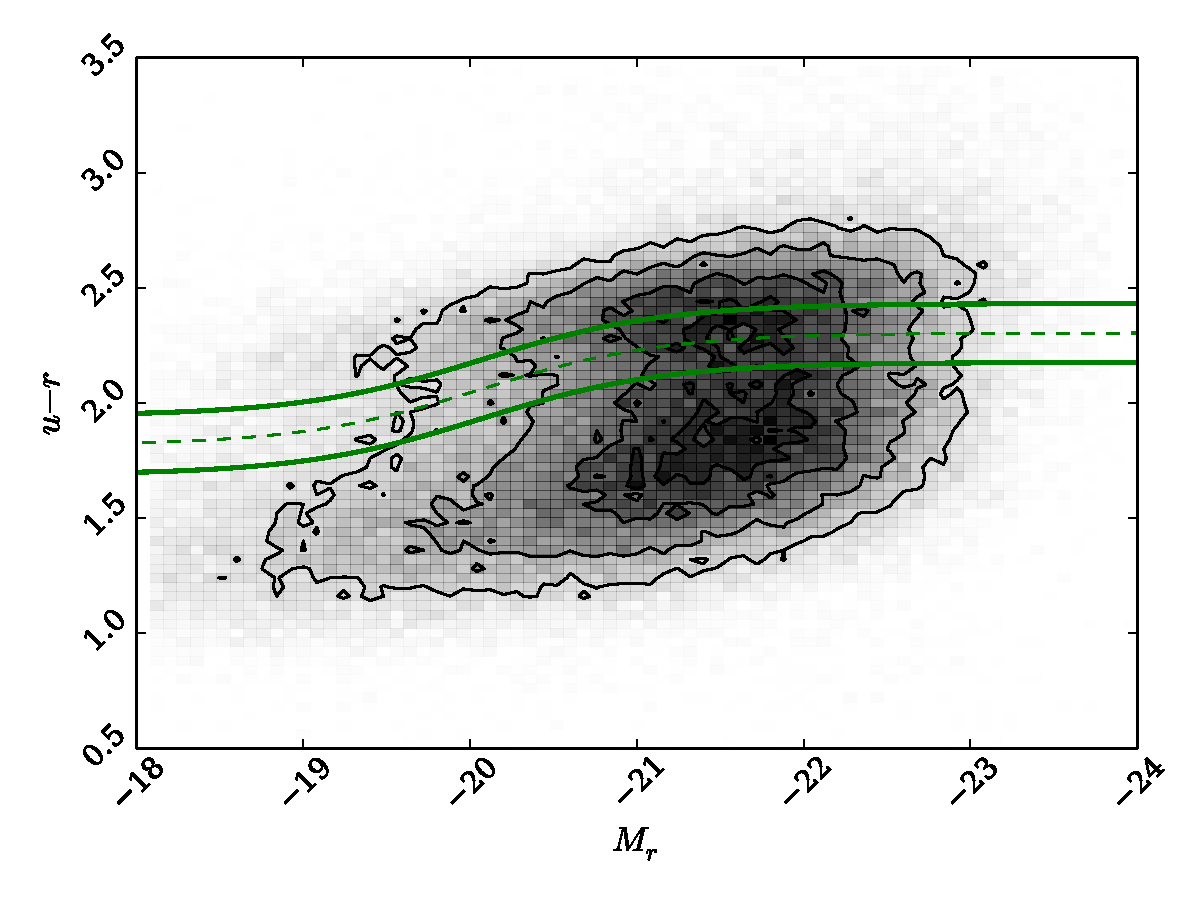
\includegraphics[width=0.45\textwidth]{col_mag_with GV.pdf}}
\caption{Colour-magnitude diagram for the GZ2 population showing the definition between the Blue Cloud and the Red Sequence from \citet{Baldry} with the dashed line. The solid lines show $\pm 1\sigma$ either side of this definition; any galaxy within the boundaries of these two solid lines is considered a Green Valley galaxy.}
\label{CMGV}
\end{figure}

\section{A Bayesian Analysis}
\subsection{Stellar Population Synthesis Models}
Using an assumed initial mass function (IMF),  stellar population synthesis models (SPS) models calculate the total flux emitted by a population, as described in \cite{BC03}

\subsection{Modelling the Star Formation History}\label{sfh}
The star formation history of a population is modelled with an exponentially declining star formation rate (SFR) at time steps from $t =0 ~Gyr$ to $t=13.7 ~Gyr$ as:

\begin{figure}
\centering{
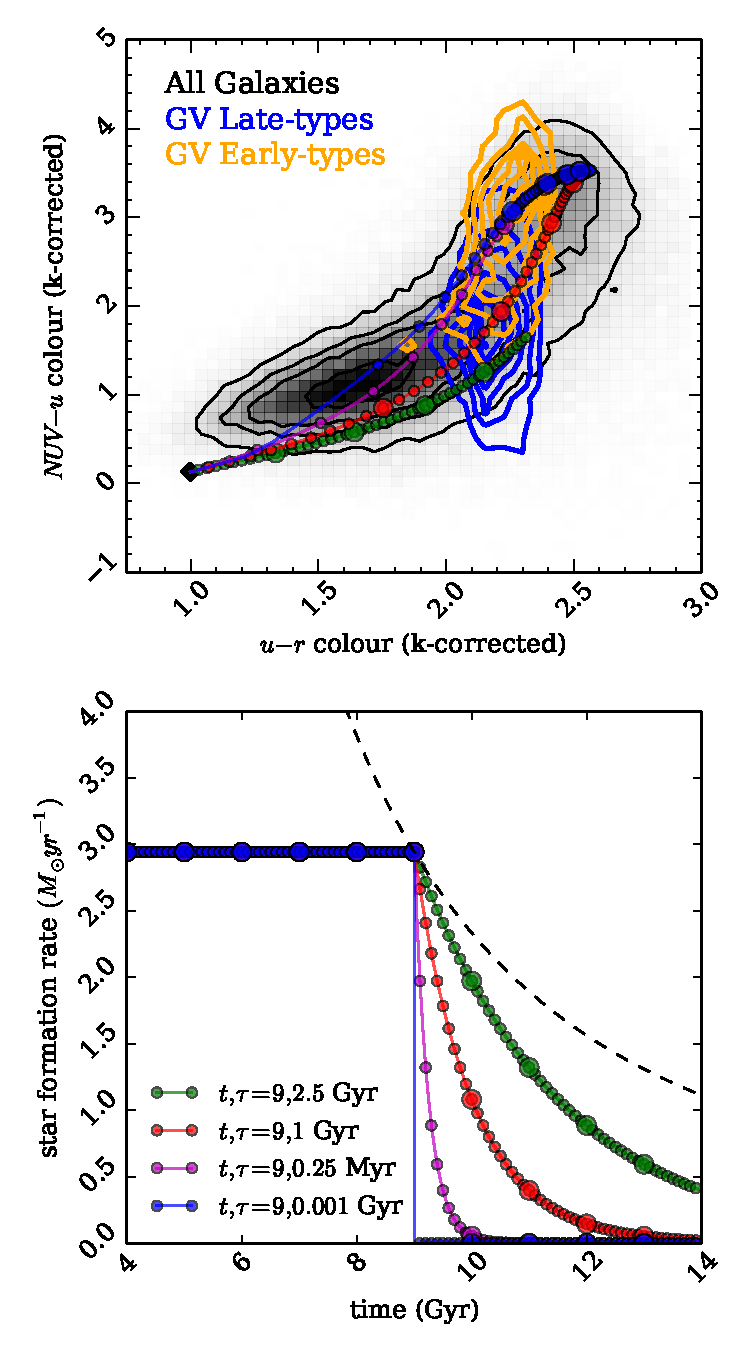
\includegraphics[width=0.45\textwidth]{kev.pdf}}
\caption{Exponentially declining star formation history models with $t_{quench}=9~Gyr$ and various $\tau$ values are shown in the bottom panel. The dashed line shows the average SFR with lookback time from \cite{Peng} which is used to set the $c_{SFR}$ at $t_{quench}$ (see section \ref{sfh}). The top panel shows the evolution with time (each point represents a time step of $1 ~Gyr$) of these models across the optical-NUV colour-colour diagram. Also shown is the distribution of the GZ2 galaxies across this colour space by the black contours.}
\label{kev}
\end{figure}


\[
SFR = 
\begin{cases}
c_{SFR} & \text{if } t < t_{q} \\
c_{SFR} \times exp{\left( \frac{-(t-t_{q})}{\tau}\right)} & \text{if } t > t_{q}
\end{cases}
\]

where $t_{q}$ is the onset time of quenching, $\tau$ is the timescale over which the quenching occurs and $c_{SFR}$ is a constant star formation rate. \citet{Peng} defined a relation in their equation 1, which is shown in their figure 3, between the average SFR and lookback time. This was used to constrain our initial constant SFR in the models; at the time $t_{q}$, the models are defined to have a SFR which lies on this relationship; see right hand panel of figure \ref{sfr_mass}. The left hand plot in figure \ref{sfr_mass} show how these models reproduce the observed relationship between the SFR and the mass of a galaxy, including how at the time of quenching they reside on the \emph{``main sequence"} of star formation, shown by the solid black line. We can also see in figure \ref{sfr_mass_evo} how this diagram evolves with cosmic time. The \emph{``main sequence"} of star formation as observed at the current epoch, is plotted in each panel in blue as a reference point. 

In our models a smaller $\tau$ value corresponds to a rapid quench (almost instantaneous suppression of star formation), whereas a large value of $\tau$ corresponds to a slower quench (slower than the dynamical timescale of a galaxy).  This model assumes that all of the populations form an initial burst of stars at $t=0$, the mass of which is set by the value of $c_{SFR}$. %The $c_{SFR}$ value is set by using the relation defined in \citet{Peng} between the average sSFR and the lookback time (i.e. redshift); at $t_{quench}$ the SFR is set to lie on this relationship (see bottom panel of figure \ref{kev}). 

Once this evolutionary SFR is obtained, we convolved it with the BC03 population synthesis models to generate a model SED for each time step. We suppress the fluxes from stars younger than $3~Myr$ to mimic the effect of birth clouds, then apply filter transmission curves to obtain AB magnitudes and therefore colours. How these colours evolve in the optical-NUV colour space can be seen in the top panel of Figure~\ref{kev}.


We can ``observe'' these model stellar populations at a given time in their history; this correlates to the lookback time at which we observe them and therefore, if they were real populations, a measurable redshift (assuming all galaxies are formed at a time $t=0$). Therefore, for each galaxy in the GZ2 sample, the lookback time was calculated from the redshift (using the \emph{cosmolopy} package provided in the Python module \emph{astroPy}) in order to compare the observed colours to the predicted models colours at that time. This lookback time $t^{lb}$ can be thought of as a galaxy's age if we assume that all galaxies formed with an initial burst of star formation at $t=0$. 

Figure \ref{pred} shows the predicted optical and NUV colours at a time of $t^{lb} = 12.8 ~Gyr$ (the average look back time of the Galaxy Zoo 2 sample) provided by the exponential SFH model. These predicted colours will be referred to as $d_{p}(t_{q}, \tau, t^{lb})$. The SFR at a time of $t^{lb}=12.8~Gyr$ is also shown in Figure \ref{pred} to compare how this correlates with the predicted colours. The $u-r$ predicted colour shows an immediate correlation with the SFR, however the $NUV-u$ colour is more sensitive to the value of $\tau$ and so is ideal for tracing any recent star formation in a population . At small $\tau$ (rapid quenching timescales) the $NUV-u$ colour is insensitive to $t_{q}$, whereas at large $\tau$ (slow quenching timescales) the colour is very sensitive to $t_{q}$. Together the two colours are ideal for tracing the effects of $t_{q}$ and $\tau$ in a population. 

\begin{figure}
\centering{
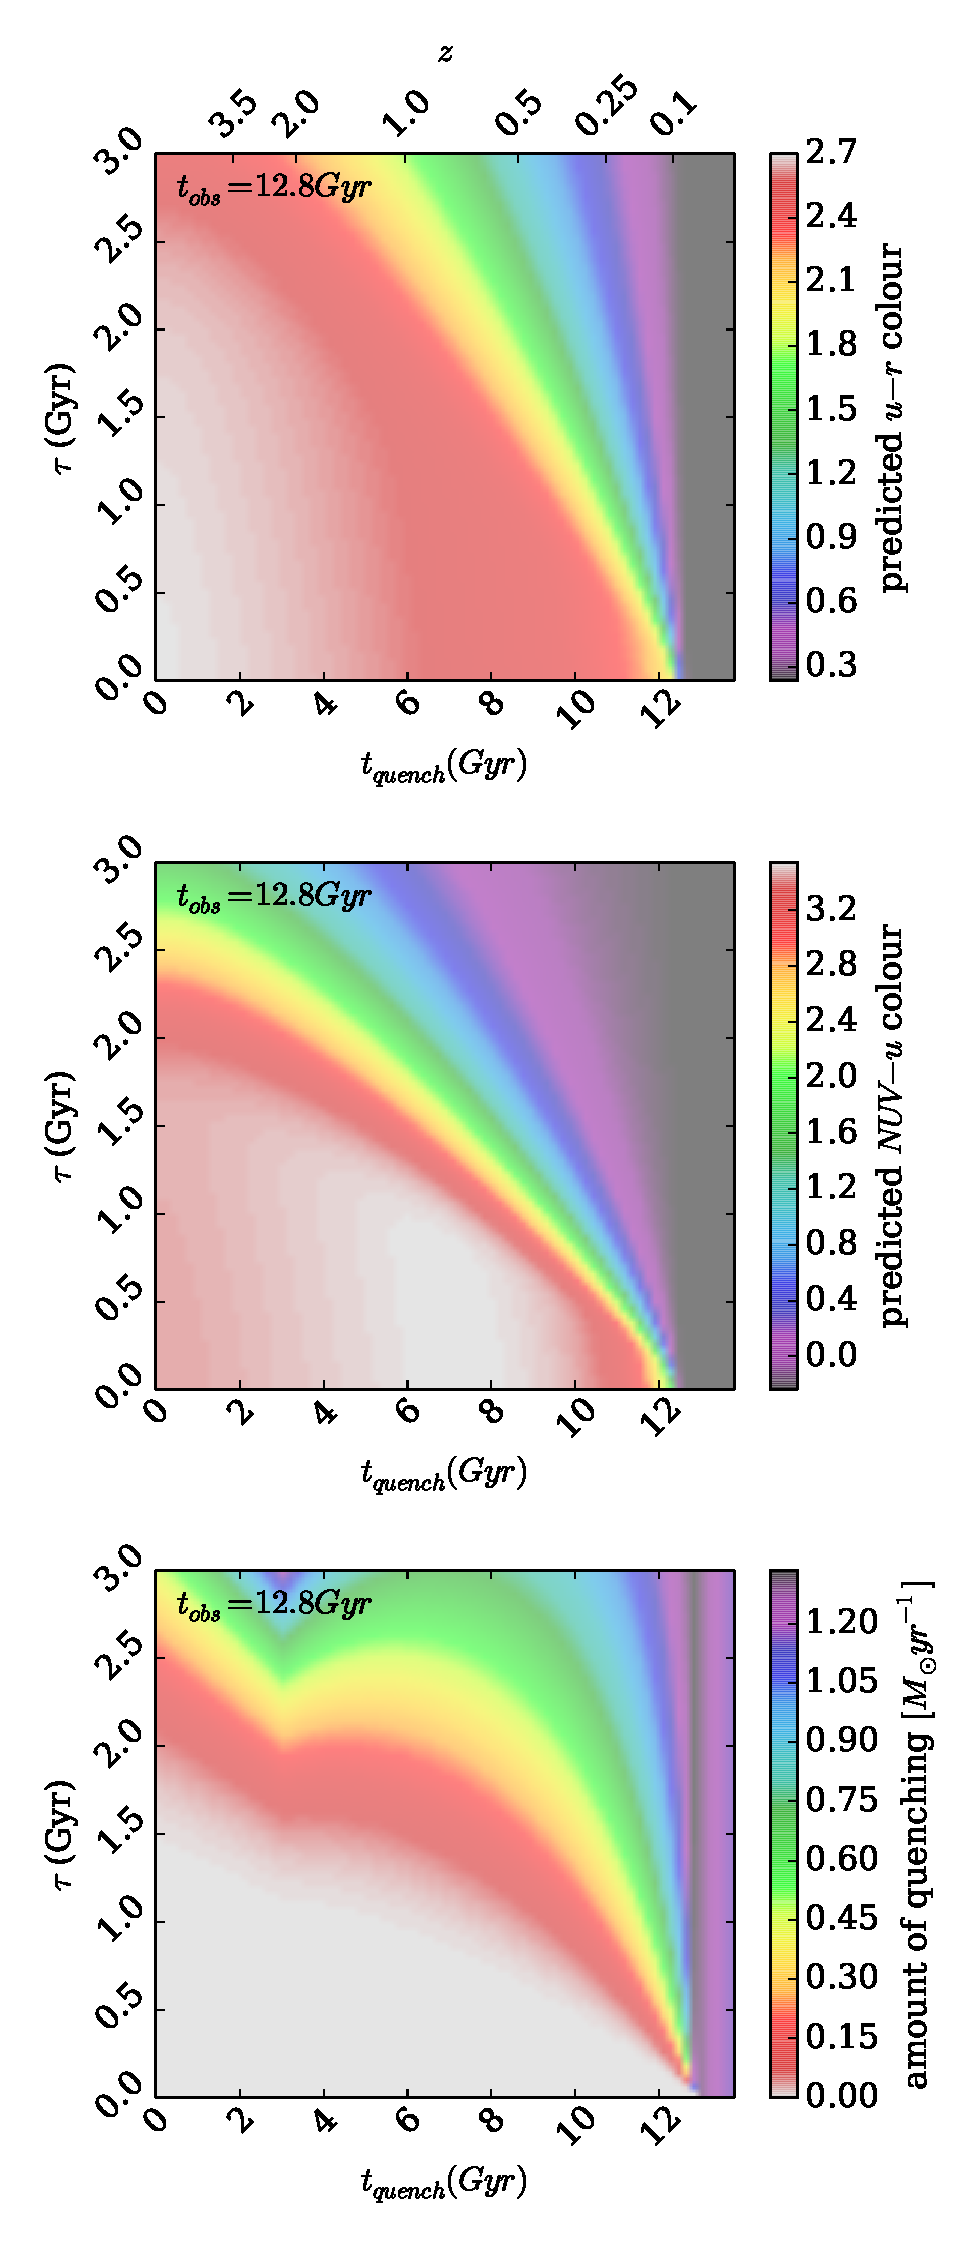
\includegraphics[width=0.45\textwidth]{colours.pdf}}
\caption{Model predictions of the $u-r$ and $NUV-u$ colours in the left and  middle panels respectively when the population is observed at $12.8~Gyr$ (the average look back time of the GZ2 sample, calculated from the observed redshift). In the right hand panel, the predicted SFR by a time of $t \sim 12.8 ~Gyr$  from the models described in sections \ref{sfh} and \ref{pengsfr}.}
\label{pred}
\end{figure}


\subsection{Bayesian Analysis}
Previous work by \citet{Sch2014} did not calculate any statistics to support their findings. Therefore to achieve robust conclusions we conducted a a fully Bayesian analysis of our SFH models in comparison to the observed GZ2 sample data. To do this we must consider all possible combinations of $(t_{q}, \tau) = \theta$ which will be distributed with a mean, $\mu$ and standard deviation, $\sigma$, so that:
\begin{equation*}
w = (\mu_{\theta}, \sigma_{\theta}) = (\mu_{t_{q}}, \sigma_{t_{q}}, \mu_{\tau}, \sigma_{\tau})
\end{equation*}
We can then define the Bayesian probability $P(\theta|w) = P(t_{q}, \tau|w) = P(t_{q}|w)P(\tau|w)$ assuming that $ P(t_{q}|w)$ and $P(\tau|w)$ are independent of each other:
\begin{multline*}
P(t_{q}, \tau|w) = \frac{1}{\sqrt[]{4\pi^2\sigma^2_{t_{q}}\sigma^2_{\tau}}} \exp\left(-\frac{(t_{q}-\mu_{t_{q}})^2}{2\sigma^2_{t_{q}}}\right) \\ \exp\left(-\frac{(\tau-\mu_{\tau})^2}{2\sigma^2_{\tau}}\right).
\end{multline*}
Which is equivalent to:
\begin{equation*}
P(\theta|w) = \frac{1}{Z_{\theta}} \exp\left(-\frac{\chi_{\theta}^2}{2}\right).
\end{equation*}
Therefore if we work in logarithmic probabilities:
\begin{equation*}
\log[P(\theta|w)] = - \log(Z_{\theta}) - \frac{\chi_{\theta}^2}{2}.
\end{equation*}
We must then find the probability of the data given these values of theta, $P(\underline{d}|\theta, t_{k}^{lb})$:
\begin{equation*}
P(\underline{d}|\theta, t_{k}^{lb}) = \prod_{k} P(d_{k}|\theta, t_{k}^{lb}),
\end{equation*}
where $d_{k}$ is a single data point (optical and NUV colours of one galaxy). We calculate $P(d_{k}|\theta, t_{k}^{lb})$ using the predicted values for the optical ($c=opt$) and NUV ($c=NUV$) colours, $d_{c,p}(\theta, t_{k}^{lb})$, for a given combination of $\theta = (t_{q}, \tau)$ and a calculated galaxy age $t^{lb}$ (look back time, calculated from a galaxy's redshift, equivalent to the age of the galaxy assuming that all galaxies formed at $t=0~Gyr$):
\begin{multline*}
P(d_{k}|\theta, t^{lb}) = \frac{1}{\sqrt{2\pi\sigma_{opt, k}^2}}\frac{1}{\sqrt{2\pi\sigma_{NUV, k}^2}} \\ \exp{\left( - \frac{(d_{opt, k} - d_{opt, p}(\theta, t_{k}^{lb}))^2}{\sigma_{opt, k}^2} \right)} \\ \exp{\left( - \frac{(d_{NUV, k} - d_{NUV, p}(\theta, t_{k}^{lb}))^2}{\sigma_{NUV, k}^2} \right)},
\end{multline*}
where for one combination of $\theta = (t_{q}, \tau)$,
\begin{equation*}
\chi_{c, k}^2 = \frac{(d_{c, k} - d_{c, p}(\theta, t_{k}^{lb}))^2}{\sigma_{c, k}^2}
\end{equation*}
and
\begin{equation*}
Z_{k} = \sqrt[]{2\pi\sigma_{c, k}^2}.
\end{equation*}
Again working in logarithmic probabilities:
\begin{equation*}
\log{(P(\underline{d}|\theta, \underline{t}^{lb}))} = \sum_{c, k} log(P(d_{c, k}|\theta, t_{k}^{lb}))
\end{equation*}
\begin{equation*}
\log{(P(\underline{d}|\theta,  \underline{t}^{lb}))}  = K - \sum_{c, k} \frac{\chi_{c, k}^2}{2},
\end{equation*}
where K is a constant:
\begin{equation*}
K = - \sum_{c, k} \log{Z_{c, k}}. 
\end{equation*}

\begin{figure*}
\centering{
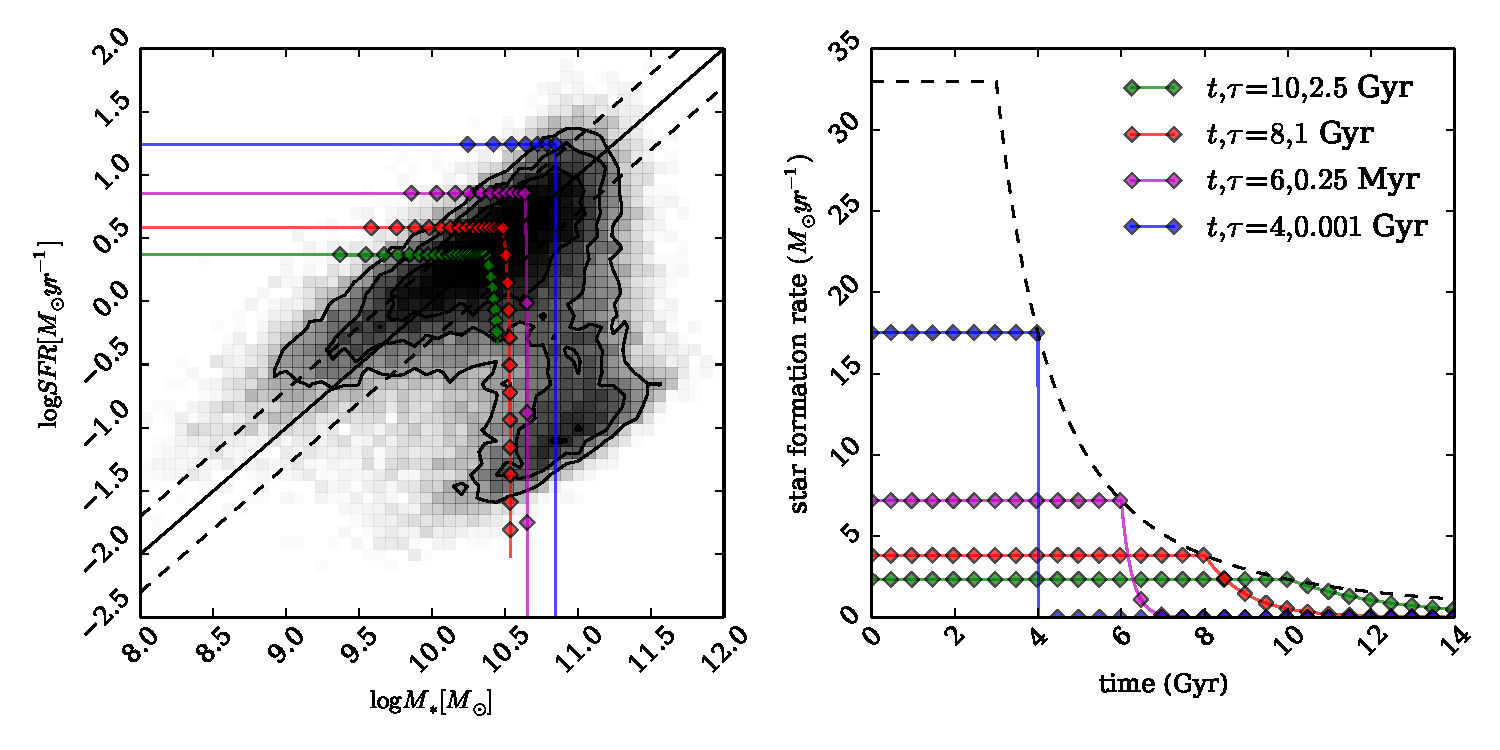
\includegraphics[width=\textwidth]{sfr_mass_diagram.pdf}}
\caption{The right hand panel shows the relationship between the star formation rate and stellar mass for the galaxies in the GZ2 sample (black contours), which trace the "main sequence" of star formation (solid line from \cite{Peng} with $\pm0.3$ dex scatter shown by the dotted lines). The SFRs and masses of the model galaxies are also shown with corresponding star formation histories shown in the left hand panel. The dashed line in the left hand panel shows the relationship between the SFR and time as defined in equation 1 of \citet{Peng}.}
\label{sfr_mass}
\end{figure*}

\begin{figure*}
\centering{
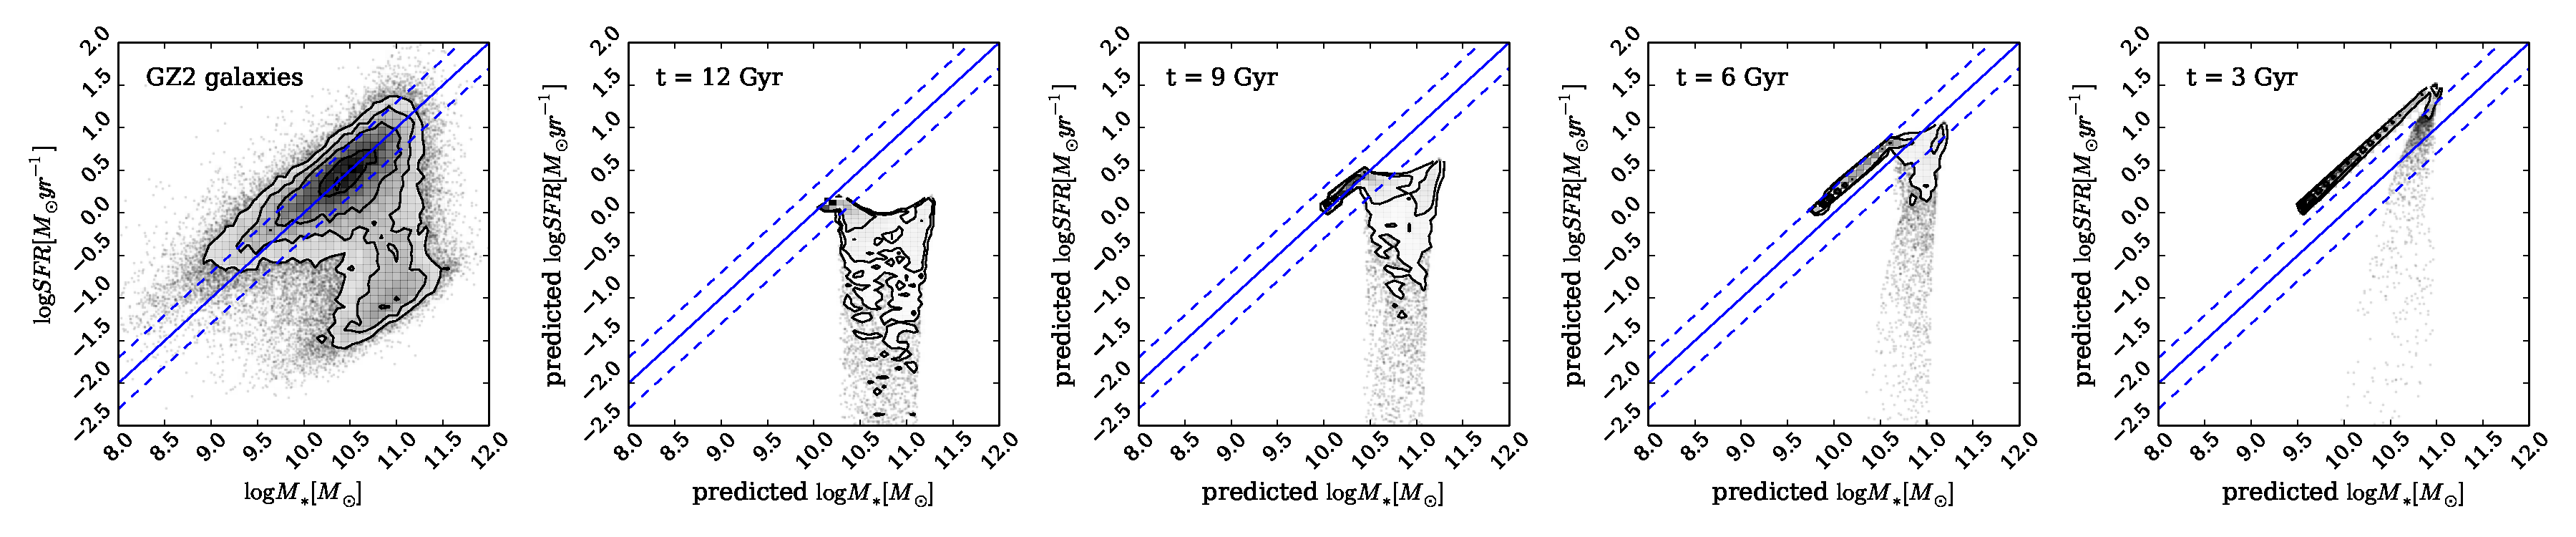
\includegraphics[width=\textwidth]{sfr_mass_evo.pdf}}
\caption{Plots to show the evolution of the SFR against the mass as predicted by the most likely exponential SFH model for each GZ2 galaxy. Each panel shows the models at different look-back times in the history of the Universe. The panel on the far left also includes the contours of the observed SFR against the mass of the GZ2 galaxies. Each panel also shows the ``main sequence'' of star formation as measured at the current epoch.}
\label{sfr_mass_evo}
\end{figure*}

\begin{figure*}
\centering{
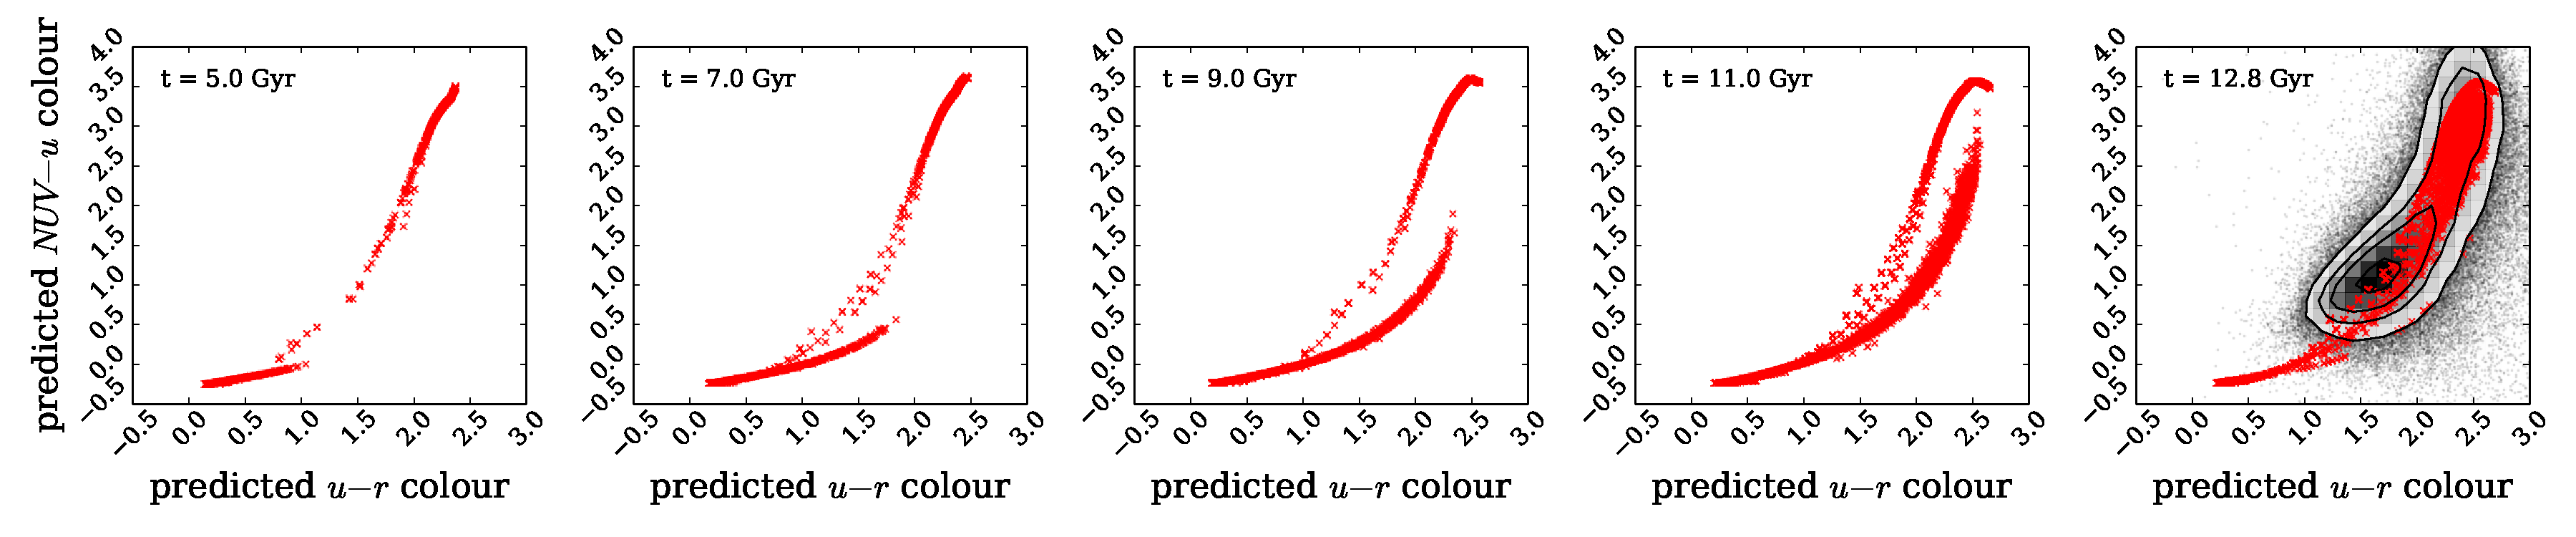
\includegraphics[width=\textwidth]{c_c_evo_numpy.pdf}}
\caption{Plots to show the evolution of the colour-colour diagram as predicted by the most likely exponential SFH model for each GZ2 galaxy. Each panel shows the model at different look-back times in the history of the Universe. The panel on the far right also includes the contours of the observed colours for the GZ2 galaxies in black, as well as the most likely predicted colours, in red, as a comparison.}
\label{c_c_evo}
\end{figure*}

What we need however is the probability of each combination of $\theta$ given the GZ2 data, $P(\theta|\underline{d})$, which we can find by:
\begin{equation*}
P(\theta|\underline{d}) = \frac{P(\underline{d}|\theta, \underline{t}^{lb})P(\theta)}{\int P(\underline{d}|\theta, \underline{t}^{lb})P(\theta) d\theta},
\end{equation*}
where,
\begin{equation*}
P(\underline{d}|\theta, \underline{t}^{lb})P(\theta) = \exp{\left[\log{[P(\underline{d}|\theta, \underline{t}^{lb})]} + \log{[P(\theta)]}\right]},
\end{equation*}
and the denominator $\int P(\underline{d}|\theta, \underline{t}^{lb})P(\theta) d\theta$ is given by the sum across all the elements of $P(\underline{d}|\theta, \underline{t}^{lb})P(\theta)$. This denominator is a mere normalisation factor, therefore when comparing the likelihoods between two different combinations of $\theta = (t_{q}, \tau)$ we need only compare the numerator and can also remain in logarithmic probability space. So given the data from the GZ2 sample, we can calculate $\log[P(\theta|\underline{d}, \underline{t}^{lb})]$ for all possible $\theta$ values and compare these to determine the most likely values for $\theta$ given the GZ2 data. In order to this robustly, we performed a Markov Chain Monte Carlo (MCMC) sampling method to cycle through the defined parameter space using a Python implementation of an affine invariant ensemble sampler \cite{Dan}; \emph{emcee}.

In addition to the colours, the GZ2 data is unique in that it provides information on a galaxy's morphology. Vote fractions from GZ2 users are available for each galaxy, for example if 80 of 100 people thought a galaxy was disc shaped, whereas 20 out of 100 people thought the same galaxy was smooth in shape (i.e. elliptical), that galaxy would have $p_{s} = 0.2$ and $p_{d} = 0.8$. In this example this galaxy would be included in the \emph{`clean'} disc sample according to \cite{GZ2}, however we loose the information that a certain majority of people classified this galaxy as \emph{smooth} (i.e. elliptical). If we just run the above sampling method on galaxies in either \emph{clean} sample, we lose any information about any intermediate galaxies and how these contribute to the likelihood of $P(\theta|\underline{d}, \underline{t}^{lb})$. It is the intermediate galaxies which are thought to be a key to the morphological changes between disc and elliptical galaxies; if this change is associated with the Green Valley in any way then these vote fractions are information we wish to keep in our sampling. 

We can incorporate these GZ2 vote fractions  into our sampling by considering them as fractions which that galaxy contributes to the likelihood $P(d_{k}|\theta)$. For example a galaxy which has $p_{s} = 0.9$ should carry more weight in the overall likelihood than a galaxy with $p_{s} = 0.1$. Therefore the likelihood can now be thought of as:
\begin{equation*}
P(\underline{d}|\theta, \underline{t}^{lb}) = \prod_{k} p_{k} P(d_{k}|\theta, t_{k}^{lb}),
\end{equation*}
where $p_{k}$ is either $p_{s}$ or $p_{d}$ for an individual galaxy. We can then feed the code with the colours for all of the GZ2 data along with first the $p_{s}$ vote fractions to find the most likely parameters for $\theta$ for elliptical galaxies and then with the $p_{d}$ vote fractions to find the most likely parameters for $\theta$ for disc galaxies. However, this is costly in computing time, therefore we perform our sampling across four parameters so that $\theta = (t_{s}, \tau_{s}, t_{d}, \tau_{d})$ and our likelihood function is then:
\begin{equation*}
P(\underline{d}|\theta, \underline{t}^{lb}) = \prod_{k} \left [p_{s, k} P(d_{k}|\theta_{s}, t_{k}^{lb}) + p_{d, k} P(d_{k}|\theta_{d}, t_{k}^{lb}) \right],
\end{equation*}
or,
\begin{equation*}
\log \left[ P(\underline{d}|\theta, \underline{t}^{lb}) \right] = \sum_{k} \log \left [p_{s, k} P(d_{k}|\theta_{s}, t_{k}^{lb}) + p_{d, k} P(d_{k}|\theta_{d}, t_{k}^{lb}) \right]. 
\end{equation*}
The code searches through the $\theta$ parameter space to find the region that then maximises $P(\theta|\underline{d})$ to return four parameter values for $t_{s}, \tau_{s}, t_{d}$ and $\tau_{d}$. If we find that $t_{s}~\sim~t{d}$ and $\tau_{s} ~\sim~ \tau{d}$ for the Green Valley galaxies then we can conclude that this area of the colour-magnitude diagram consists of  single population. 




\section{Results}

\begin{figure*}
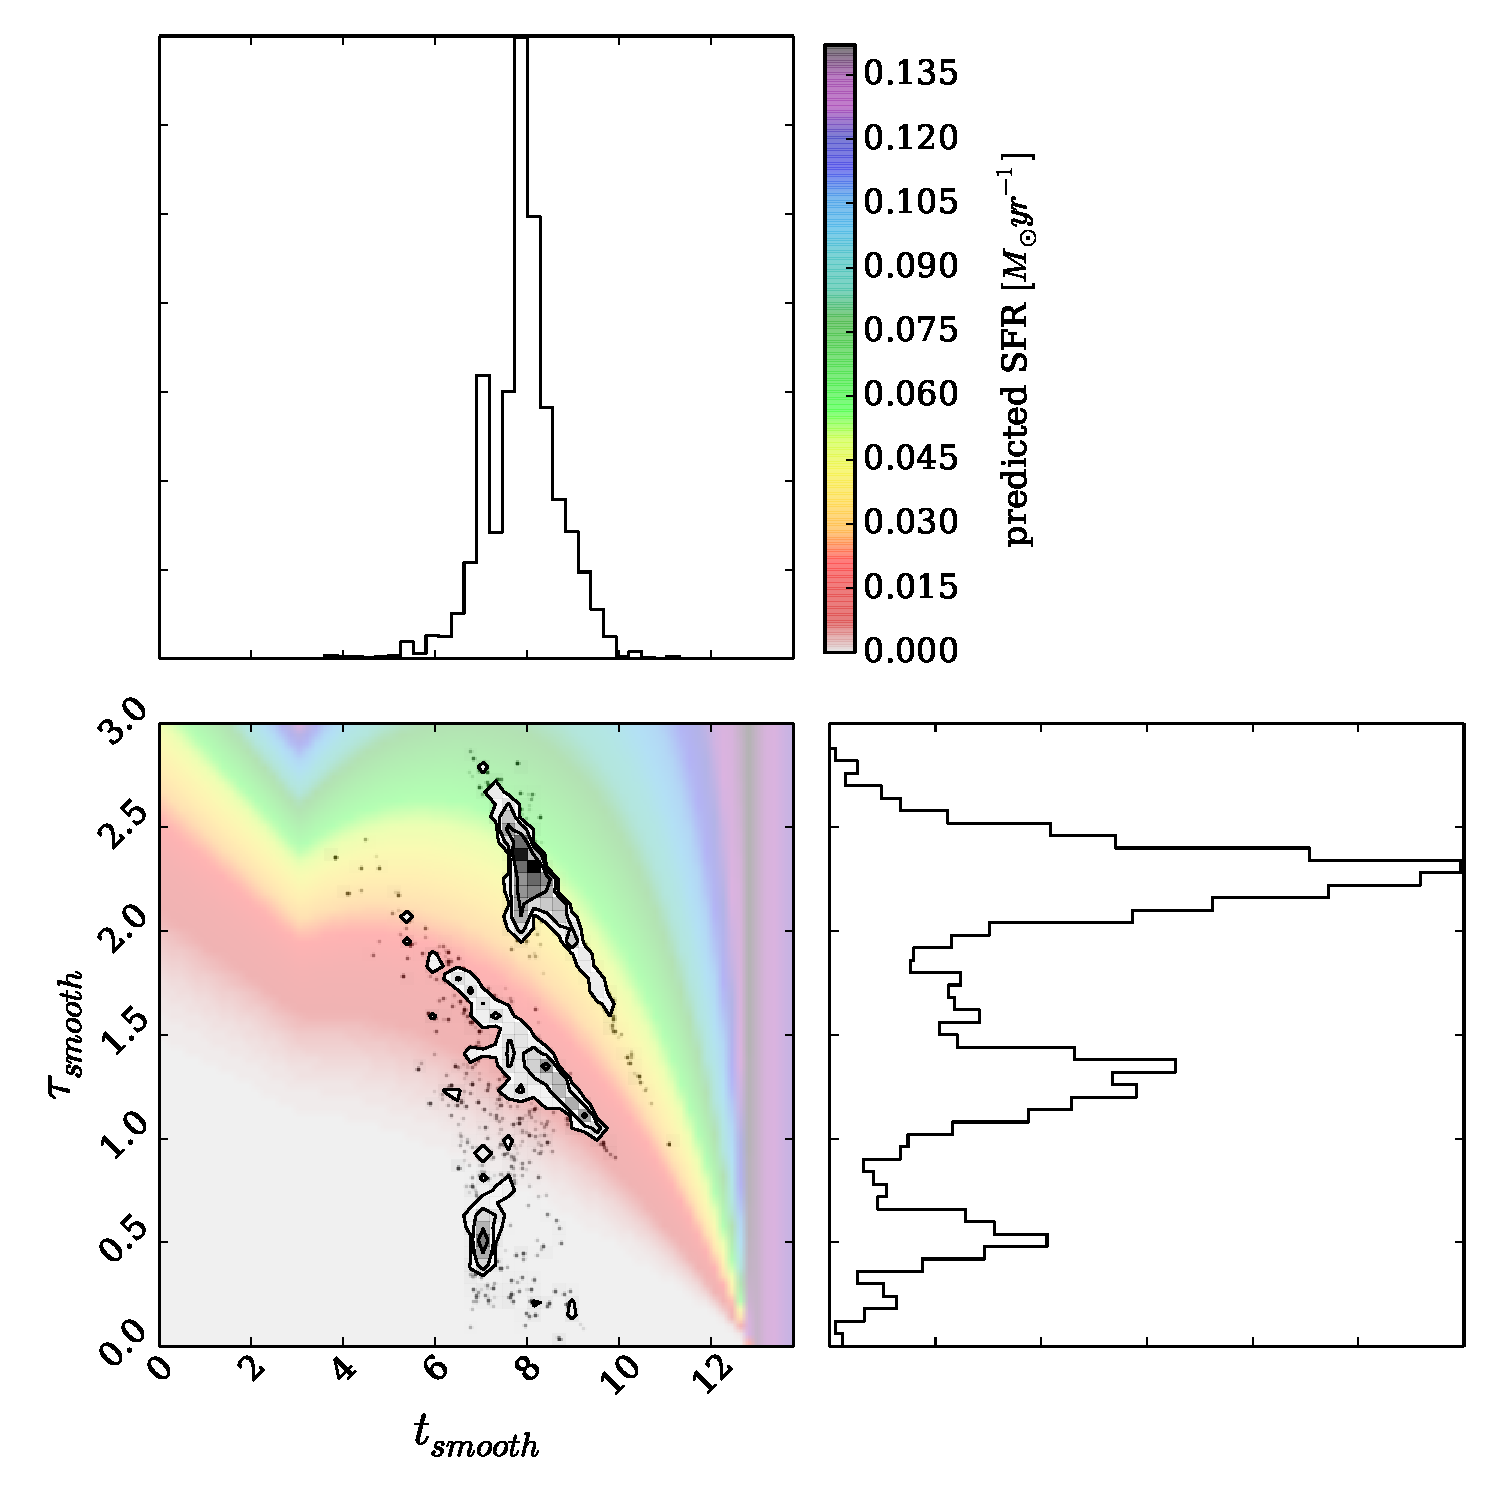
\includegraphics[width=0.4975\textwidth]{all_smooth.pdf}
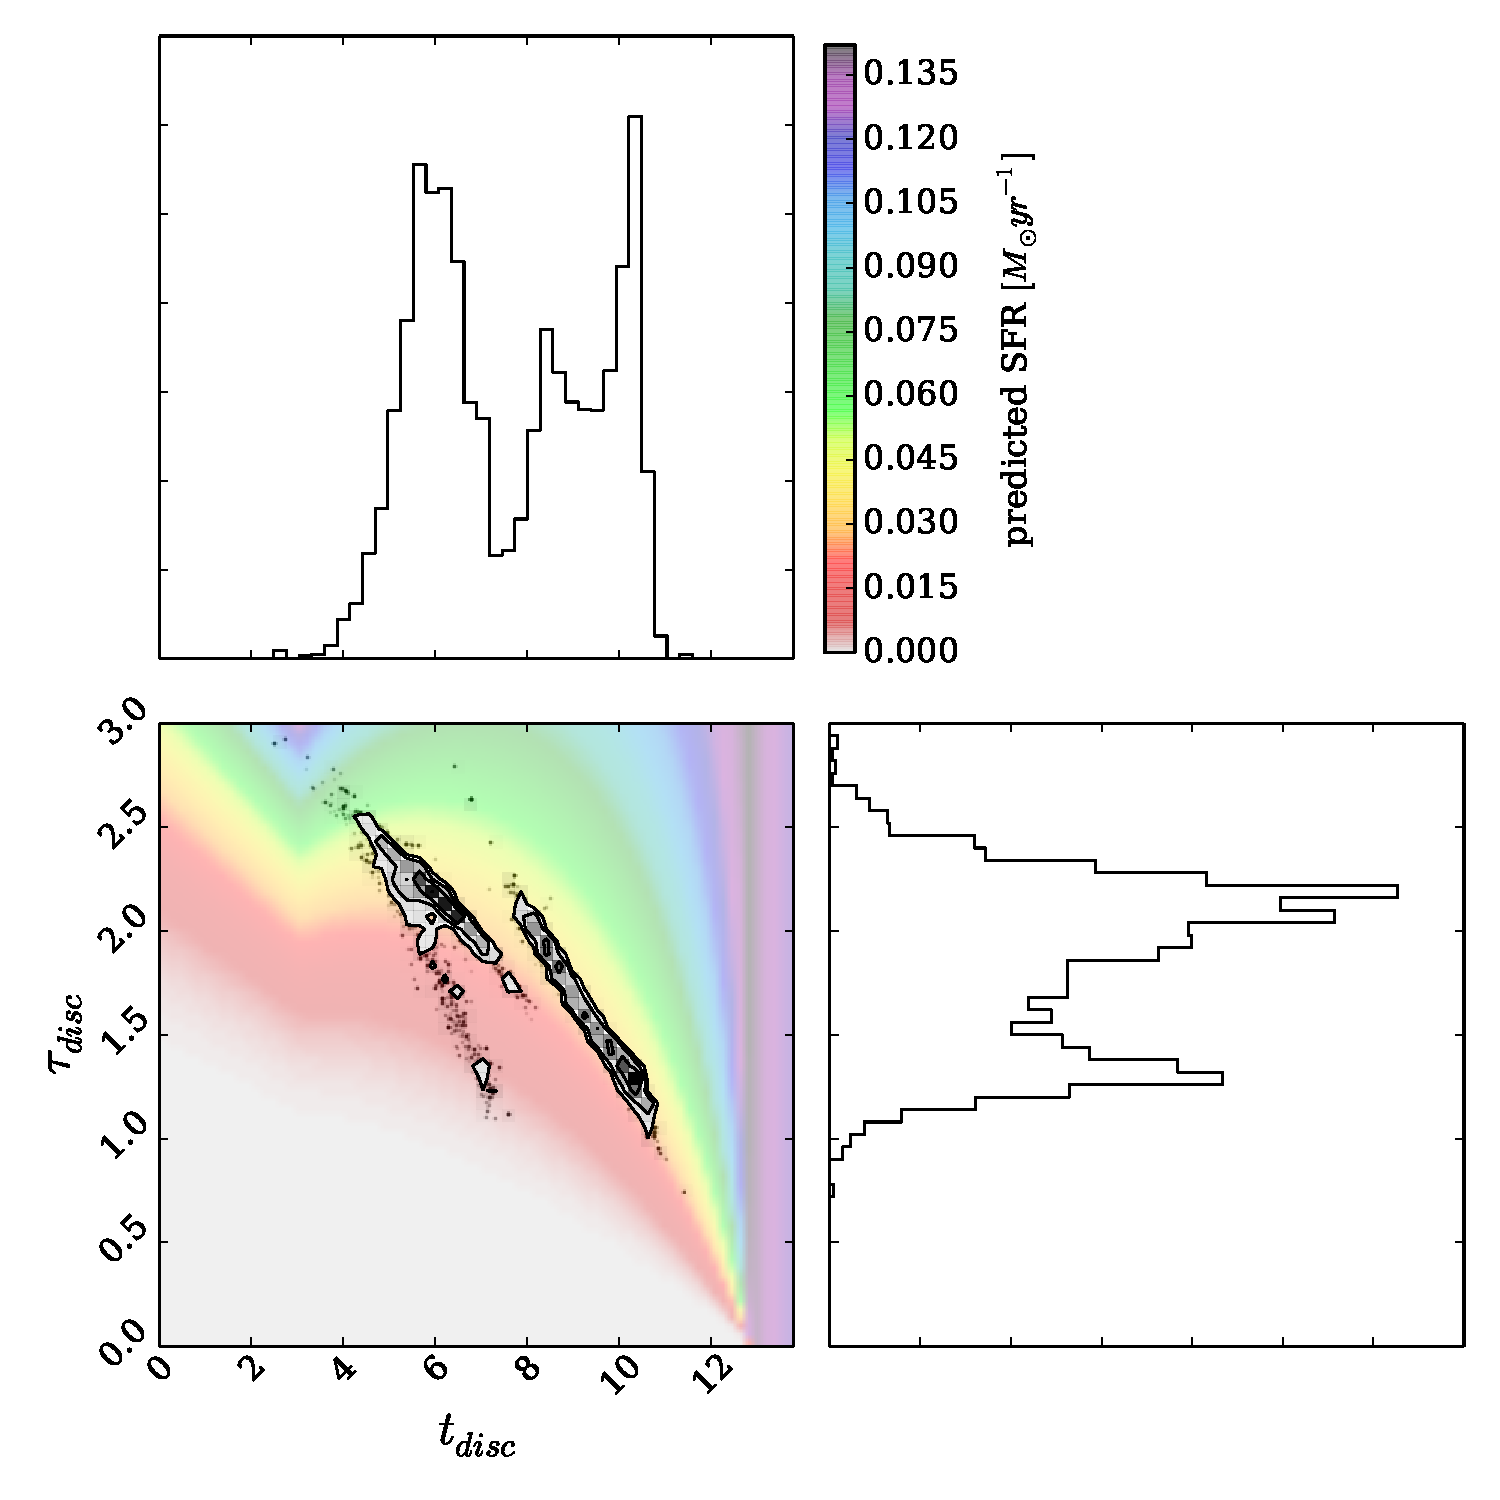
\includegraphics[width=0.4975\textwidth]{all_disc.pdf}
\caption[8pt]{For all the galaxies in the Galaxy Zoo 2 sample, contour and histogram plots show the regions of greatest likelihood for an exponential model star formation history parameters $[t_{quench}$ and $\tau_{quench}]$ for both smooth-like(left) and disc-like (right) galaxies. $t_{q}$ is the time at which quenching occurs (Gyr) and $\tau_{q}$ is the time scale on which quenching occurs (Gyr; the larger the $\tau_{q}$, the slower the quenching). Background colours show the star formation rate predicted by this model after a time $t \sim 12.8~Gyr$, which is the mean look back time of the galaxies in the GZ2 sample. Galaxies contribute  to $[t_{q}, \tau_{q}]_{smooth}$ and $[t_{q}, \tau_{q}]_{disc}$ according to their Galaxy Zoo 2 vote fraction (i.e. a galaxy with $p_{disc} \sim p_{smooth} \sim 0.5$ will contribute equally to each set of parameters).}
\label{all}
\end{figure*}


The contour plots that follow show the regions of high likelihood for the various samples of galaxies of the SFH parameters outlined in section \ref{sfh}, produced using an MCMC sampling method. It is expected that those subsets of galaxies with large numbers will rapidly converge the \emph{`walkers'} into the regions of high likelihood without the need to explore the whole parameter space. Conversely the smaller galaxy subsets will allow a full exploration of the parameter space. It is also expected that those subsets of galaxies with narrow ranges of either NUV or optical colours will also cause the \emph{`walkers'} to converge rapidly into the regions of high likelihood without the need to explore the whole of the parameter space.


This raises the issue of whether the sampling method is capable of finding multiple likelihood peaks, however the figures below show that this is not the case. 

\begin{figure*}
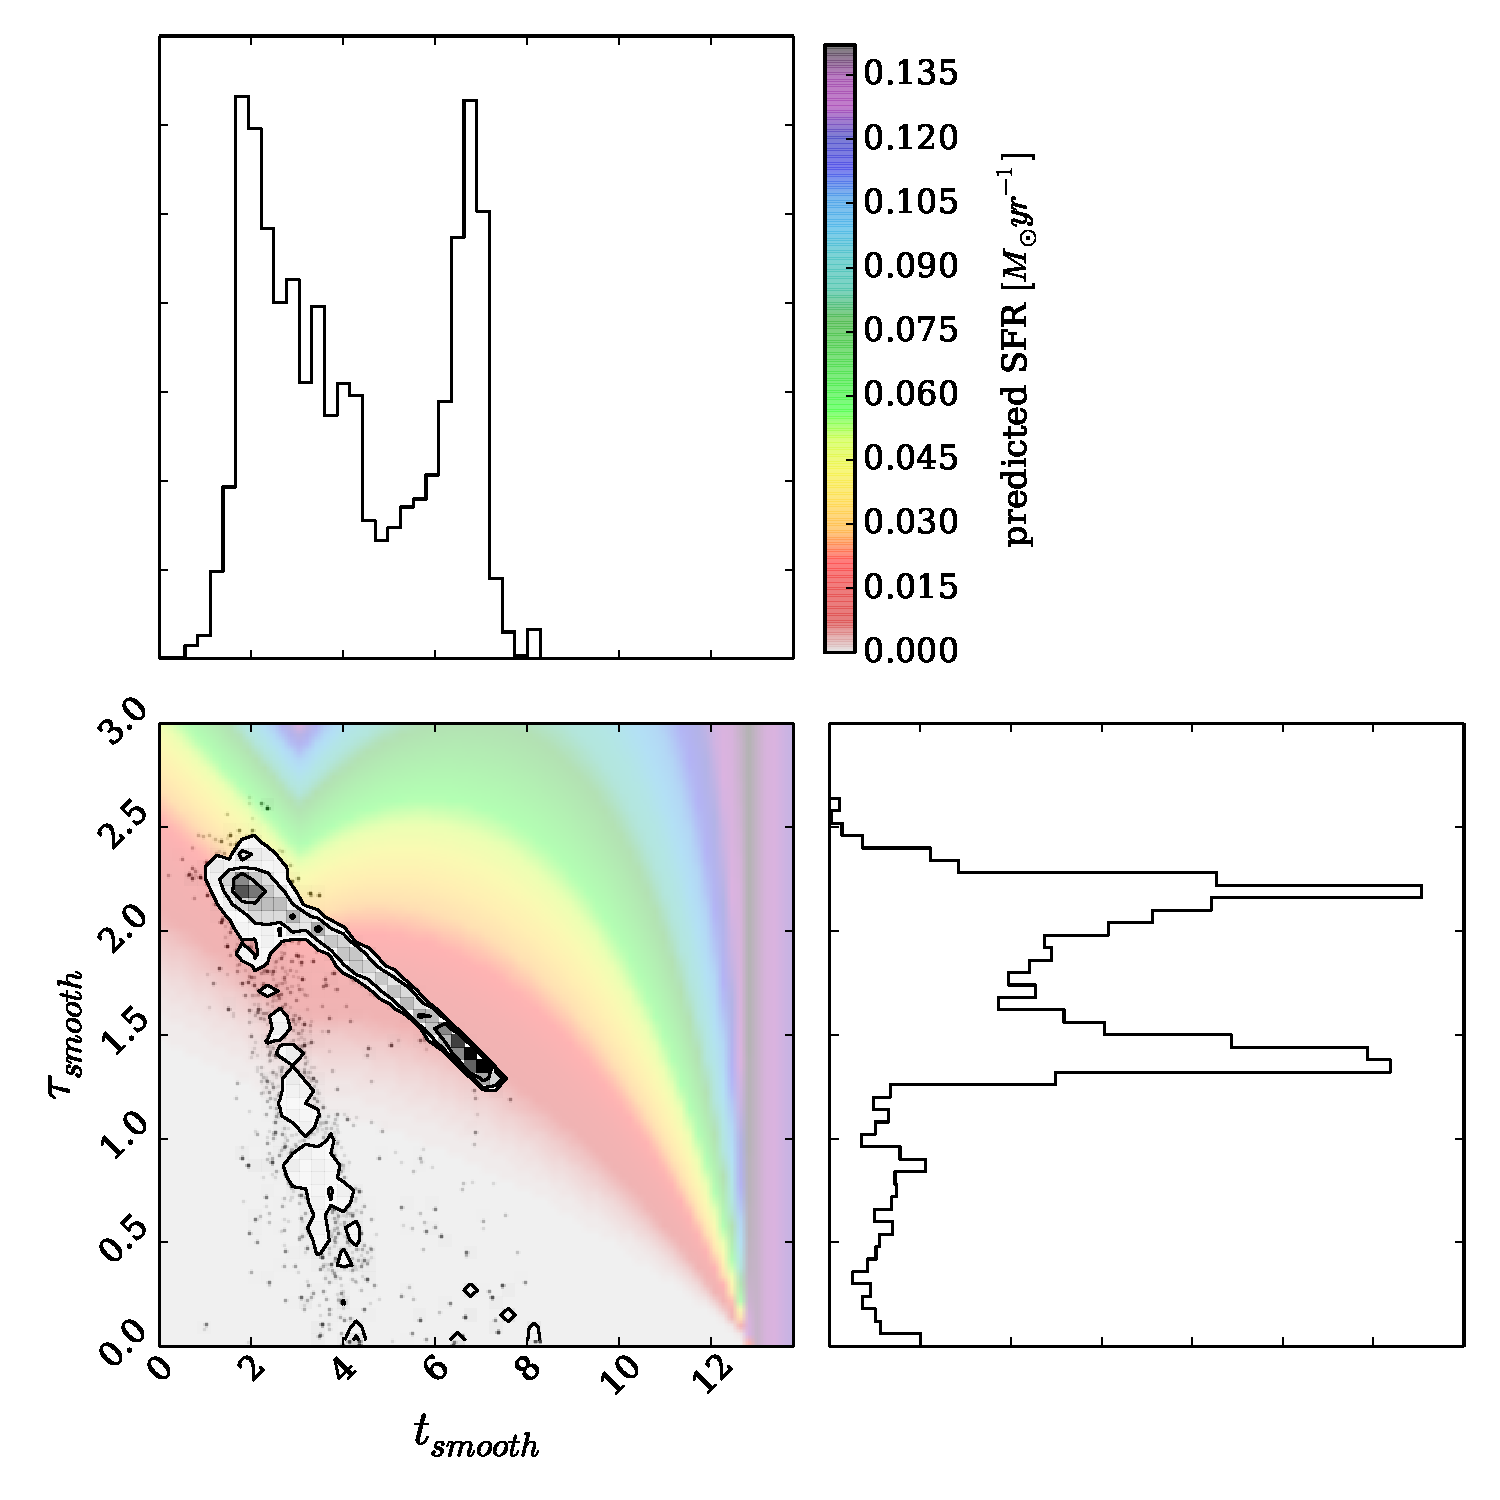
\includegraphics[width=0.4975\textwidth]{red_s_smooth.pdf}
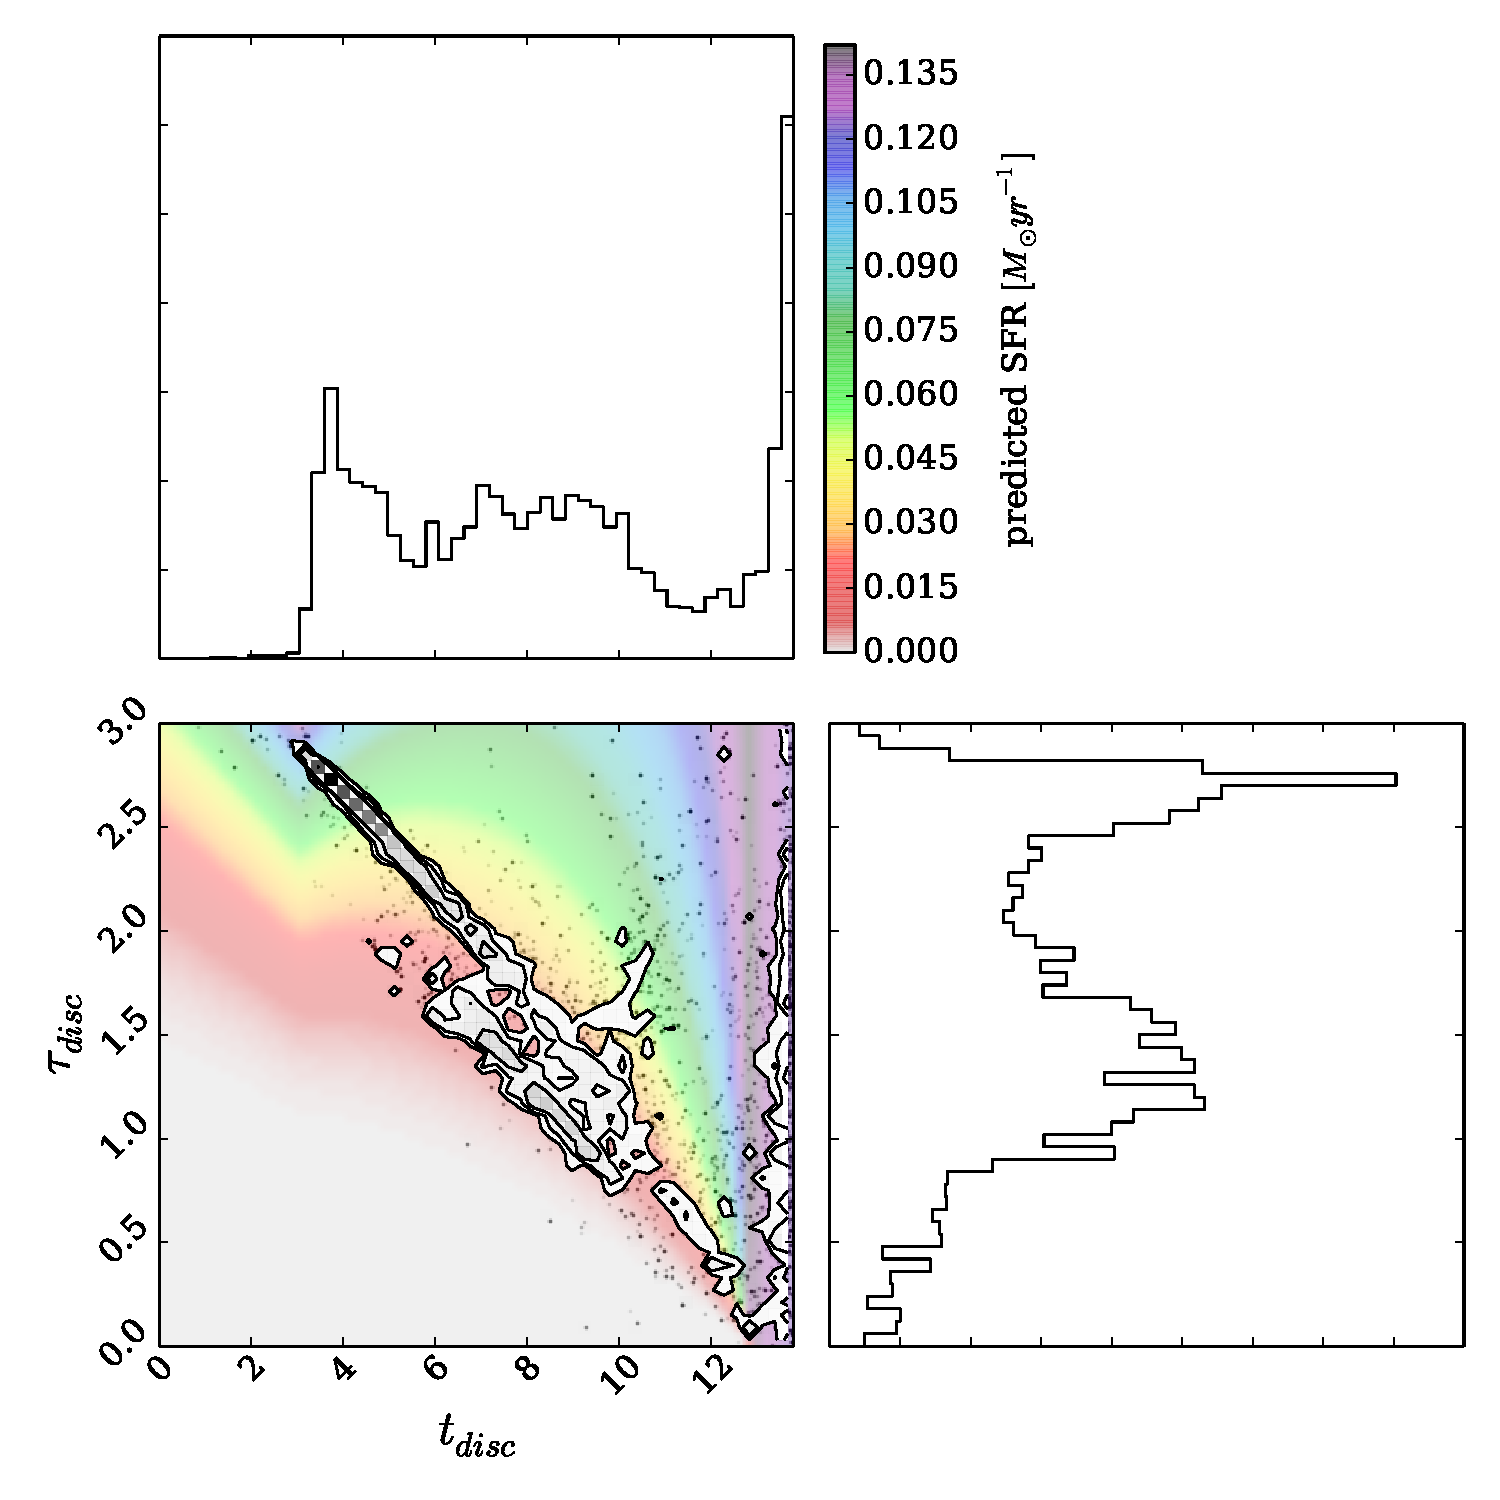
\includegraphics[width=0.4975\textwidth]{red_s_disc.pdf}
\caption[8pt]{Same as for Figure \ref{all} but for galaxies defined as optical Red Sequence \cite{Baldry}.}
\label{red_s}
\end{figure*}

\begin{figure*}
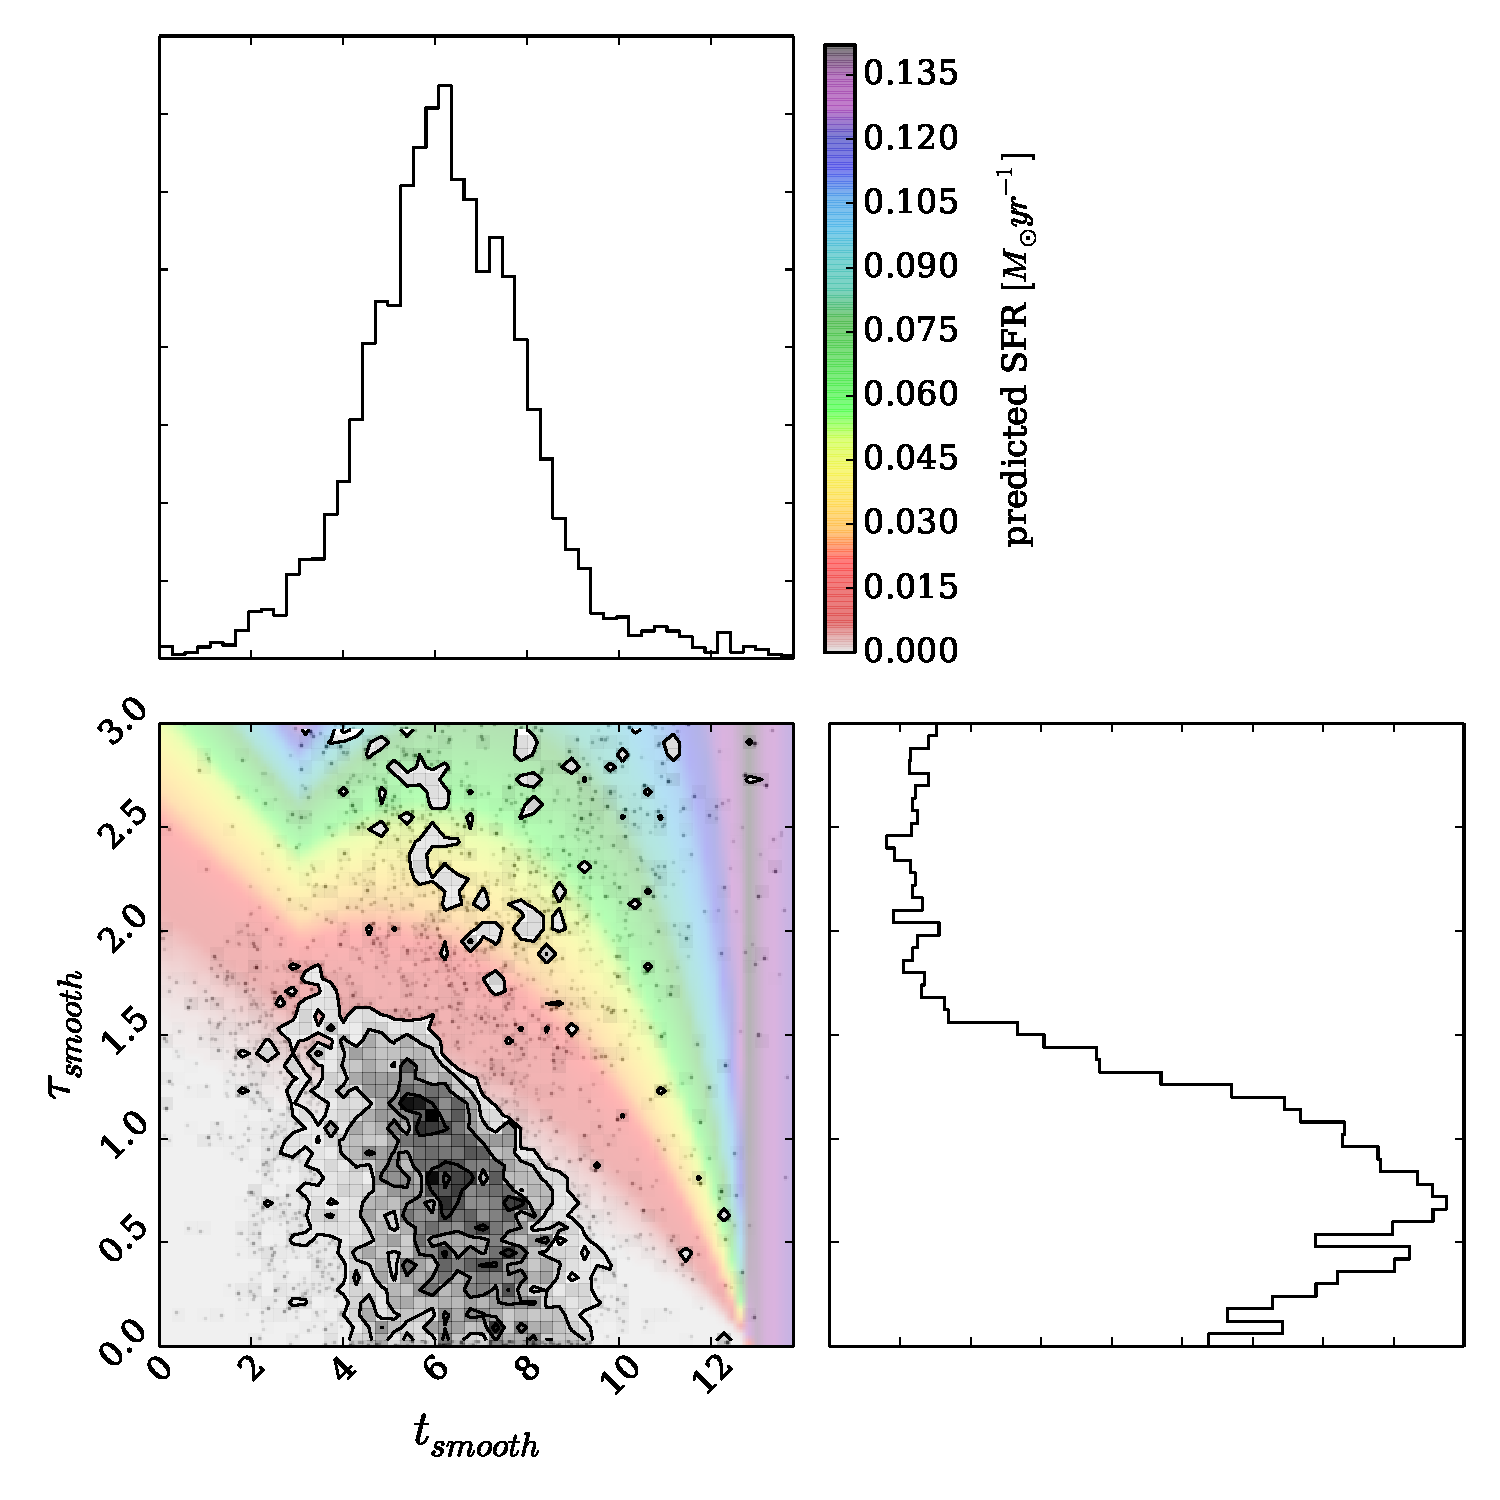
\includegraphics[width=0.4975\textwidth]{red_s_smooth_clean.pdf}
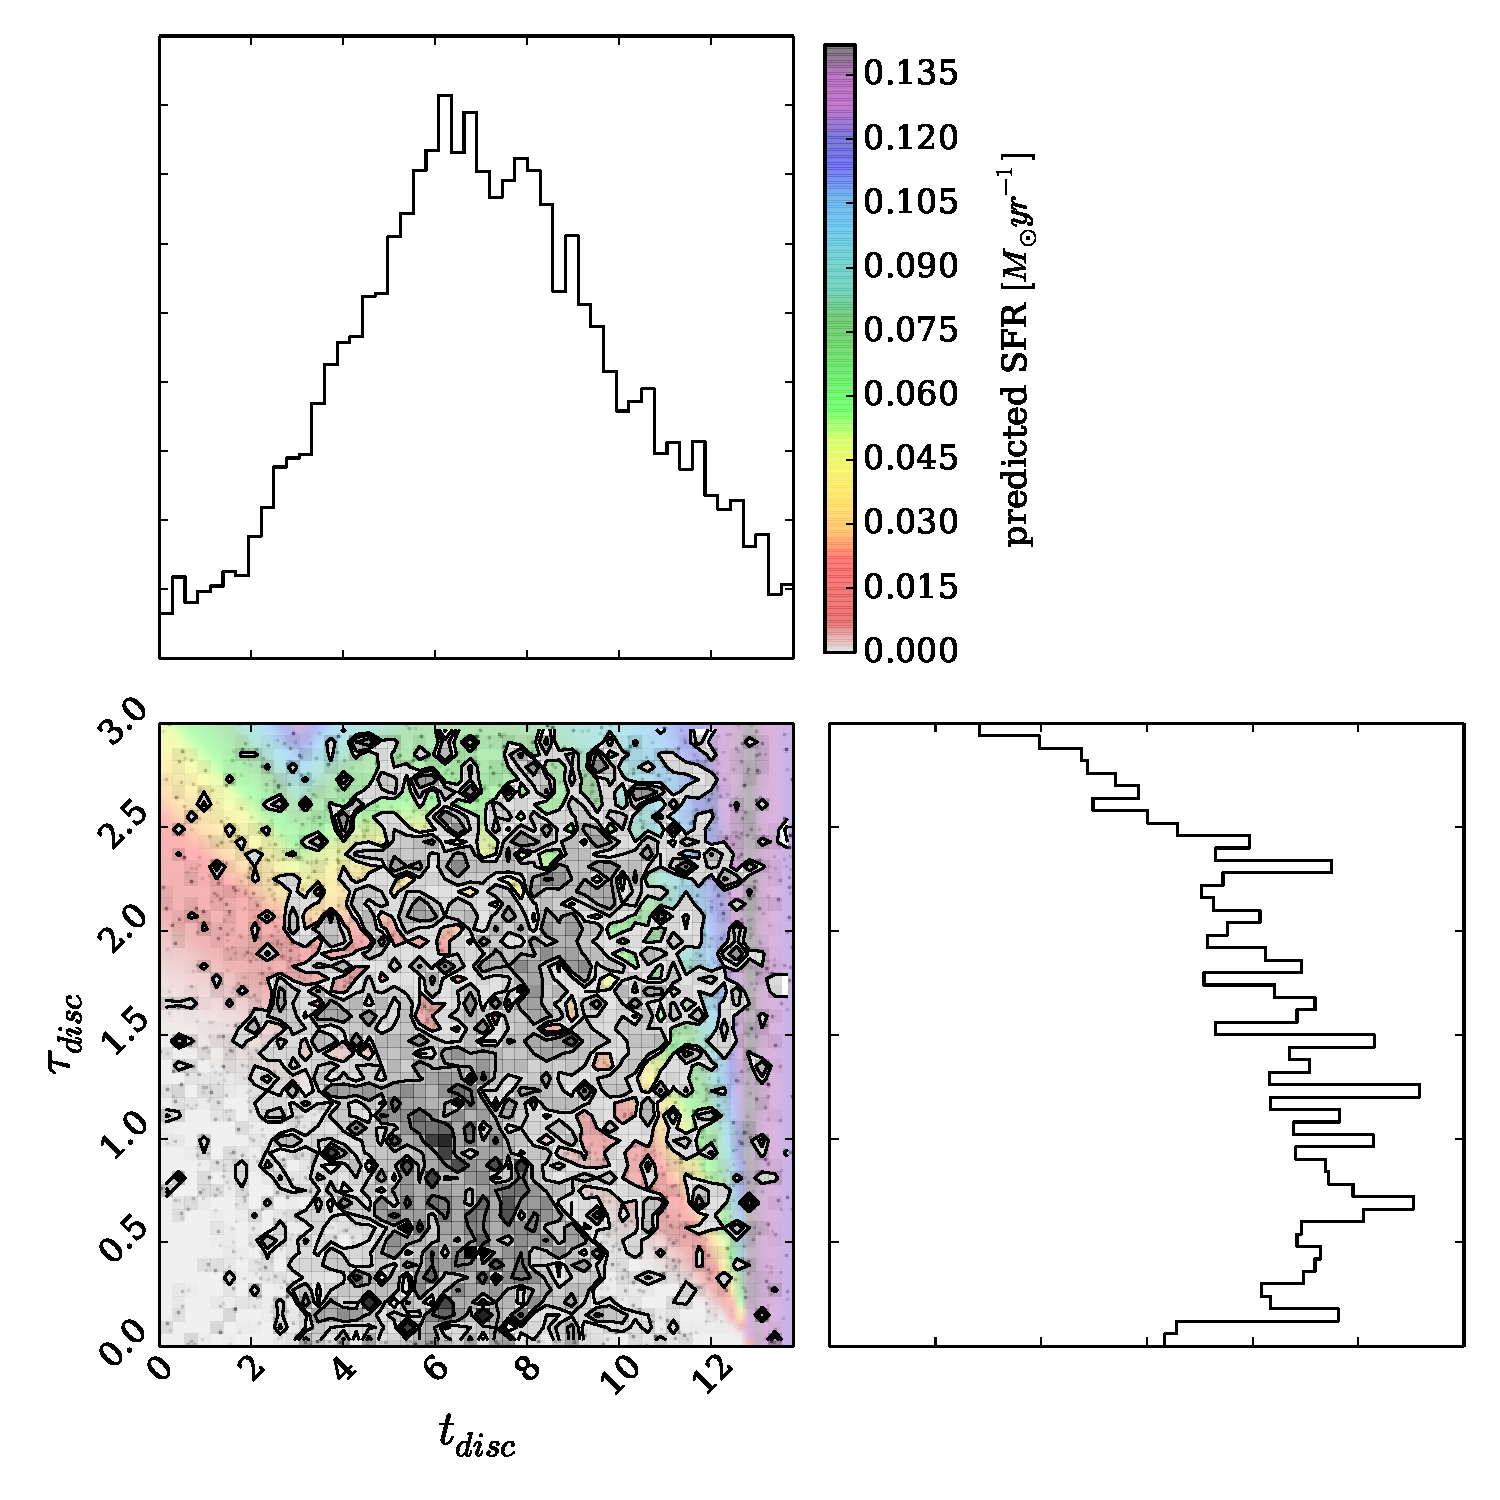
\includegraphics[width=0.4975\textwidth]{red_s_disc_clean.pdf}
\caption{Same as for Figure \ref{all} but for galaxies from the clean sample and defined as optical Red Sequence \cite{Baldry}.}
\label{red_s_clean}
\end{figure*}

\begin{figure*}
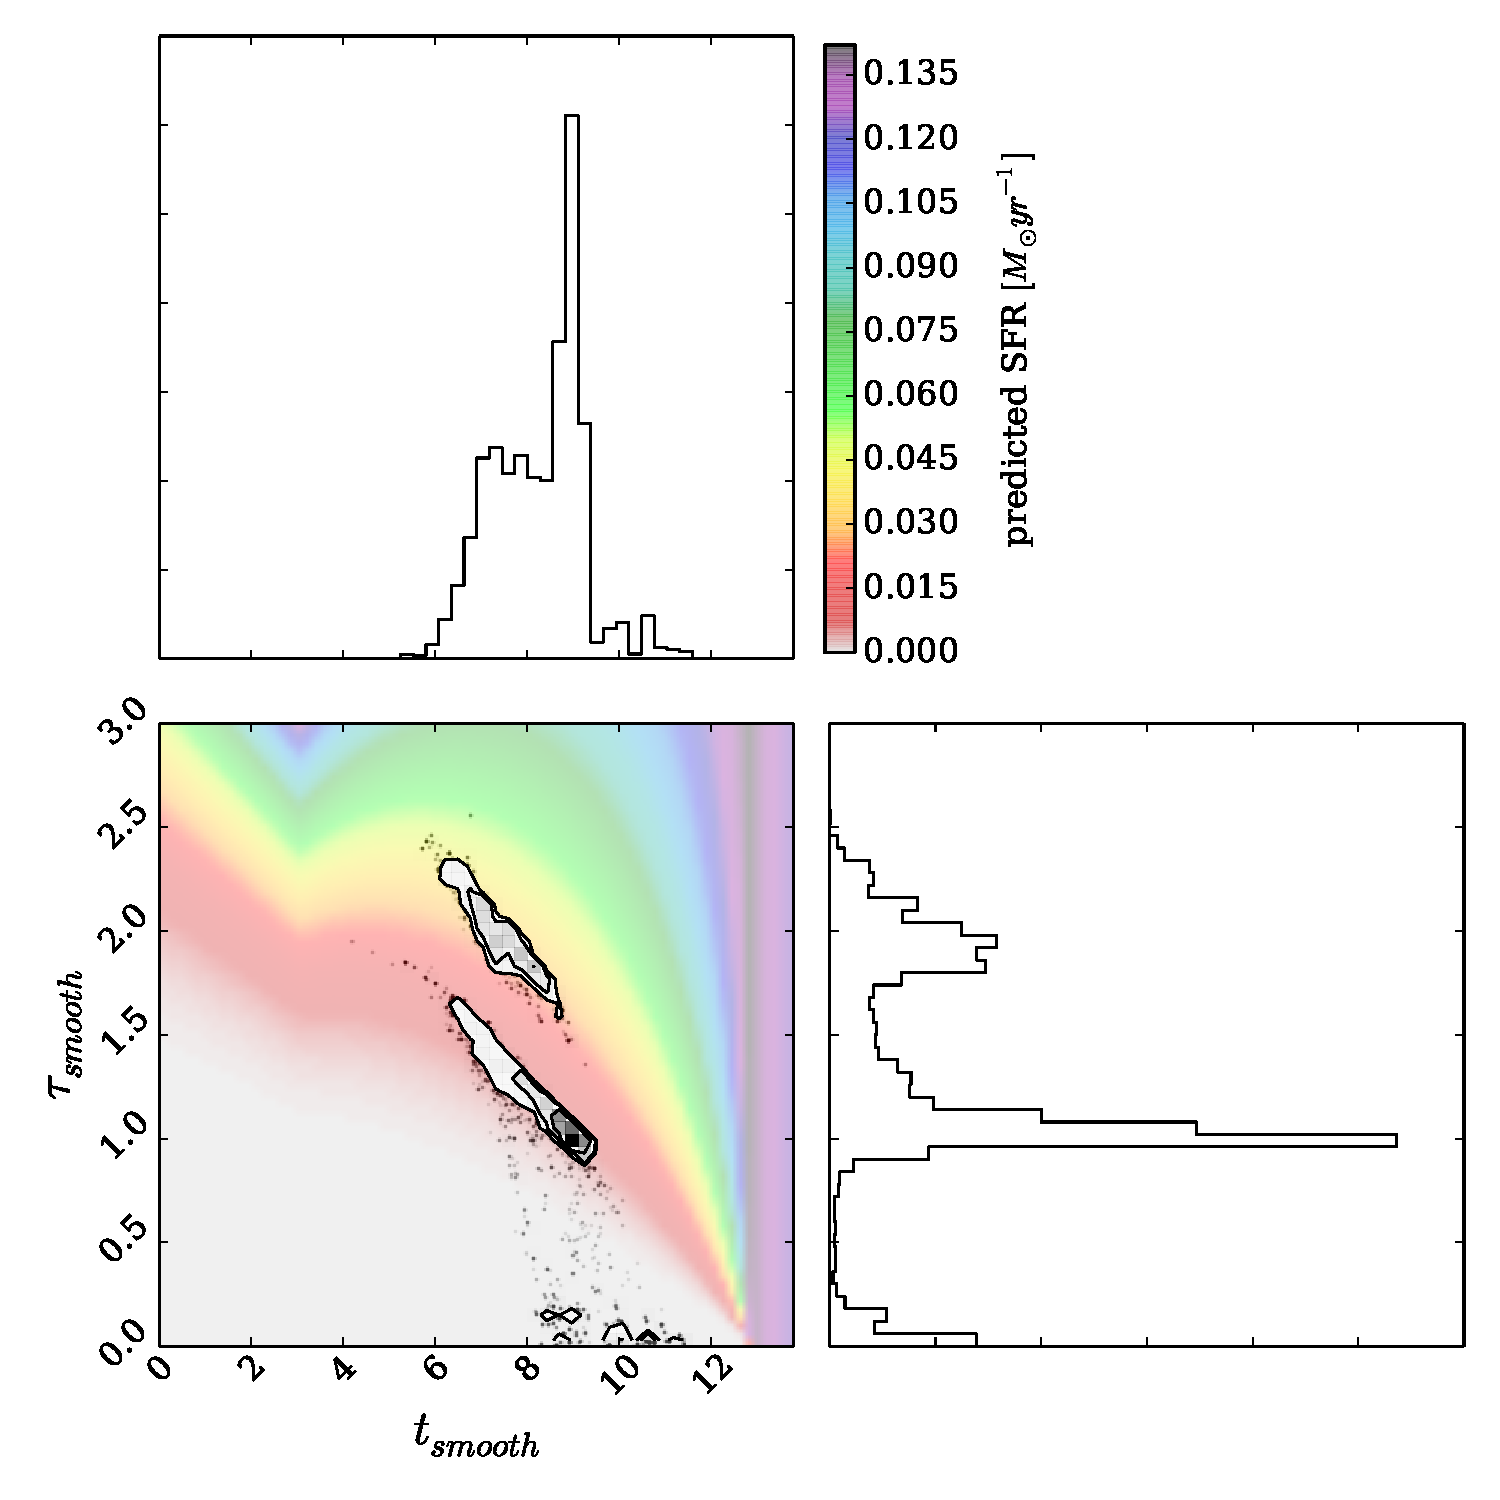
\includegraphics[width=0.4975\textwidth]{gv_smooth.pdf}
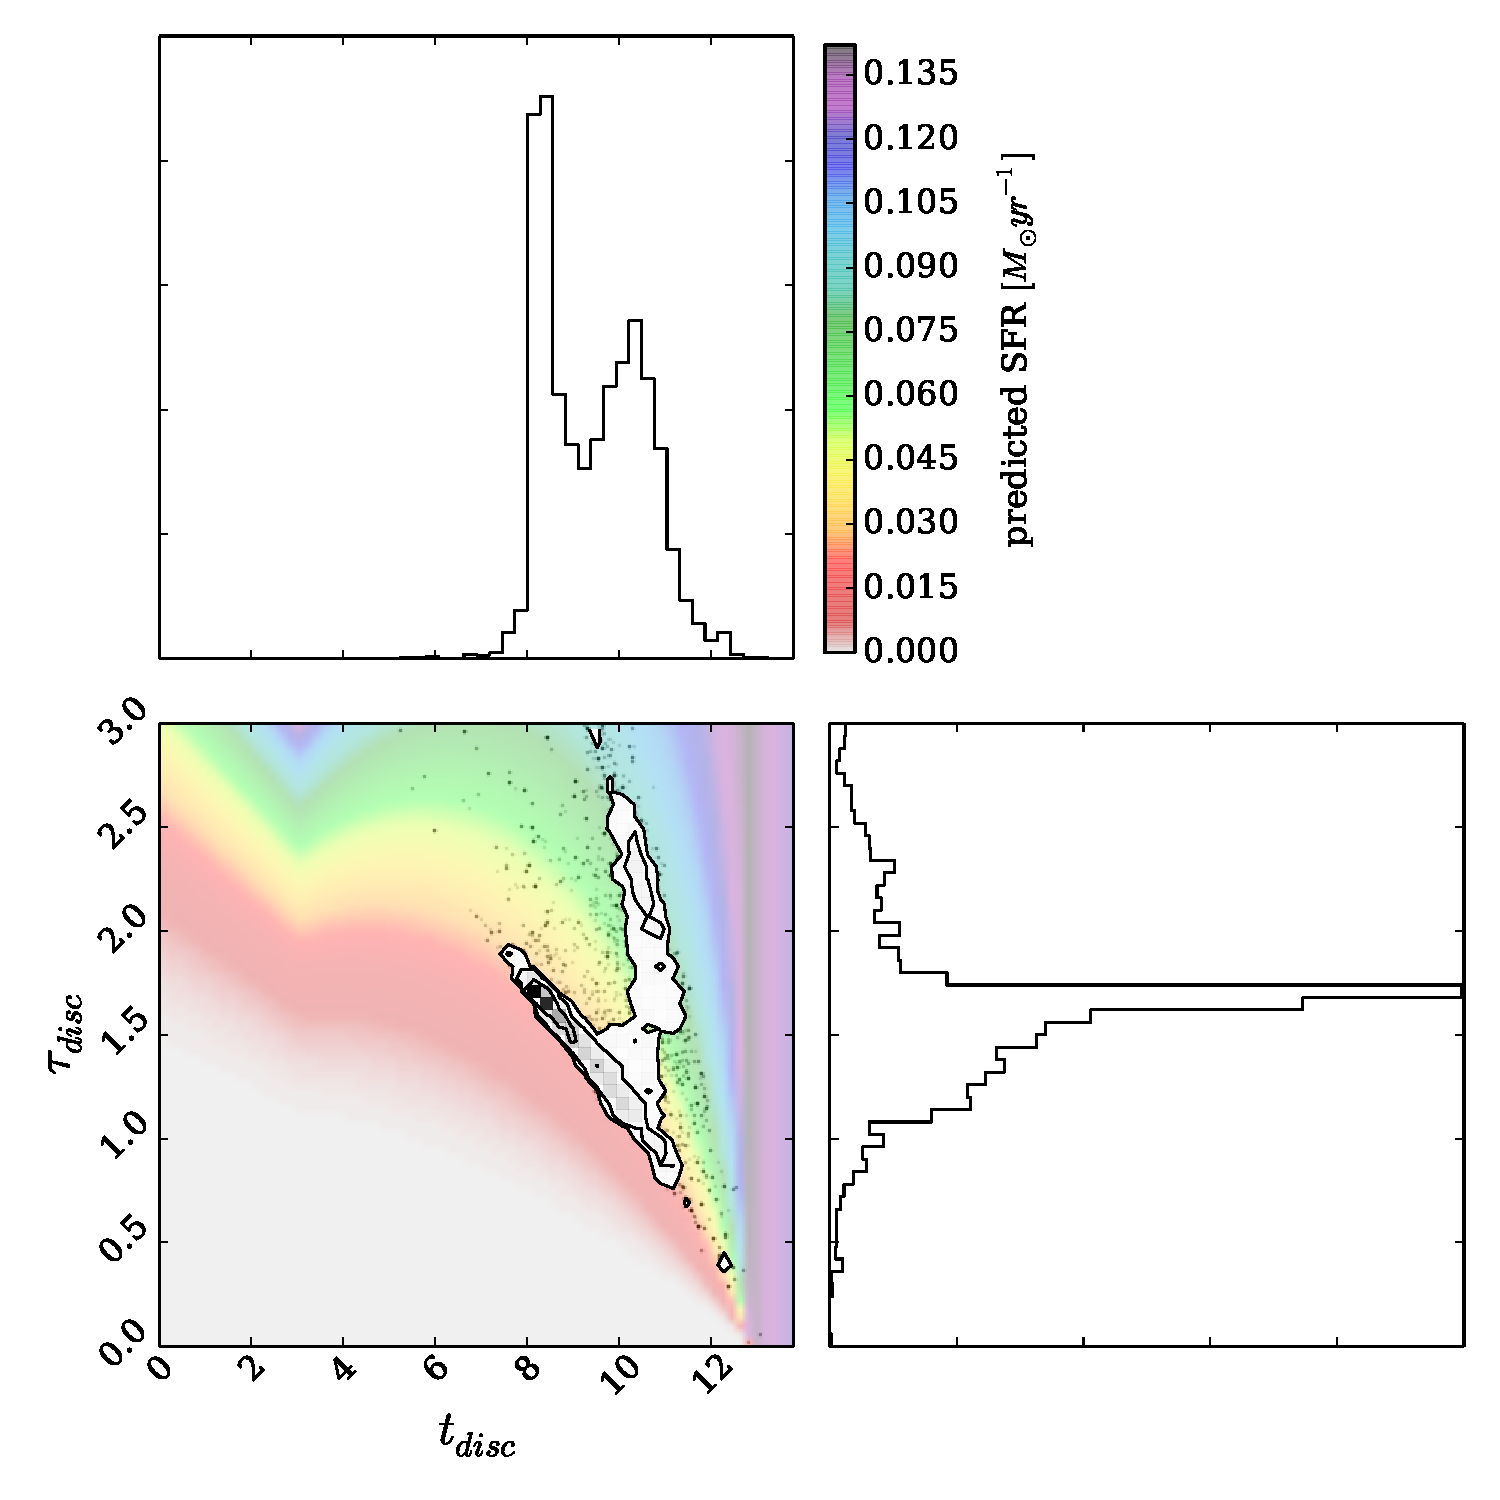
\includegraphics[width=0.4975\textwidth]{gv_disc.pdf}
\caption{Same as for Figure \ref{all} but for galaxies defined as optical Green Valley \cite{Baldry}.}
\label{gv}
\end{figure*}

\begin{figure*}
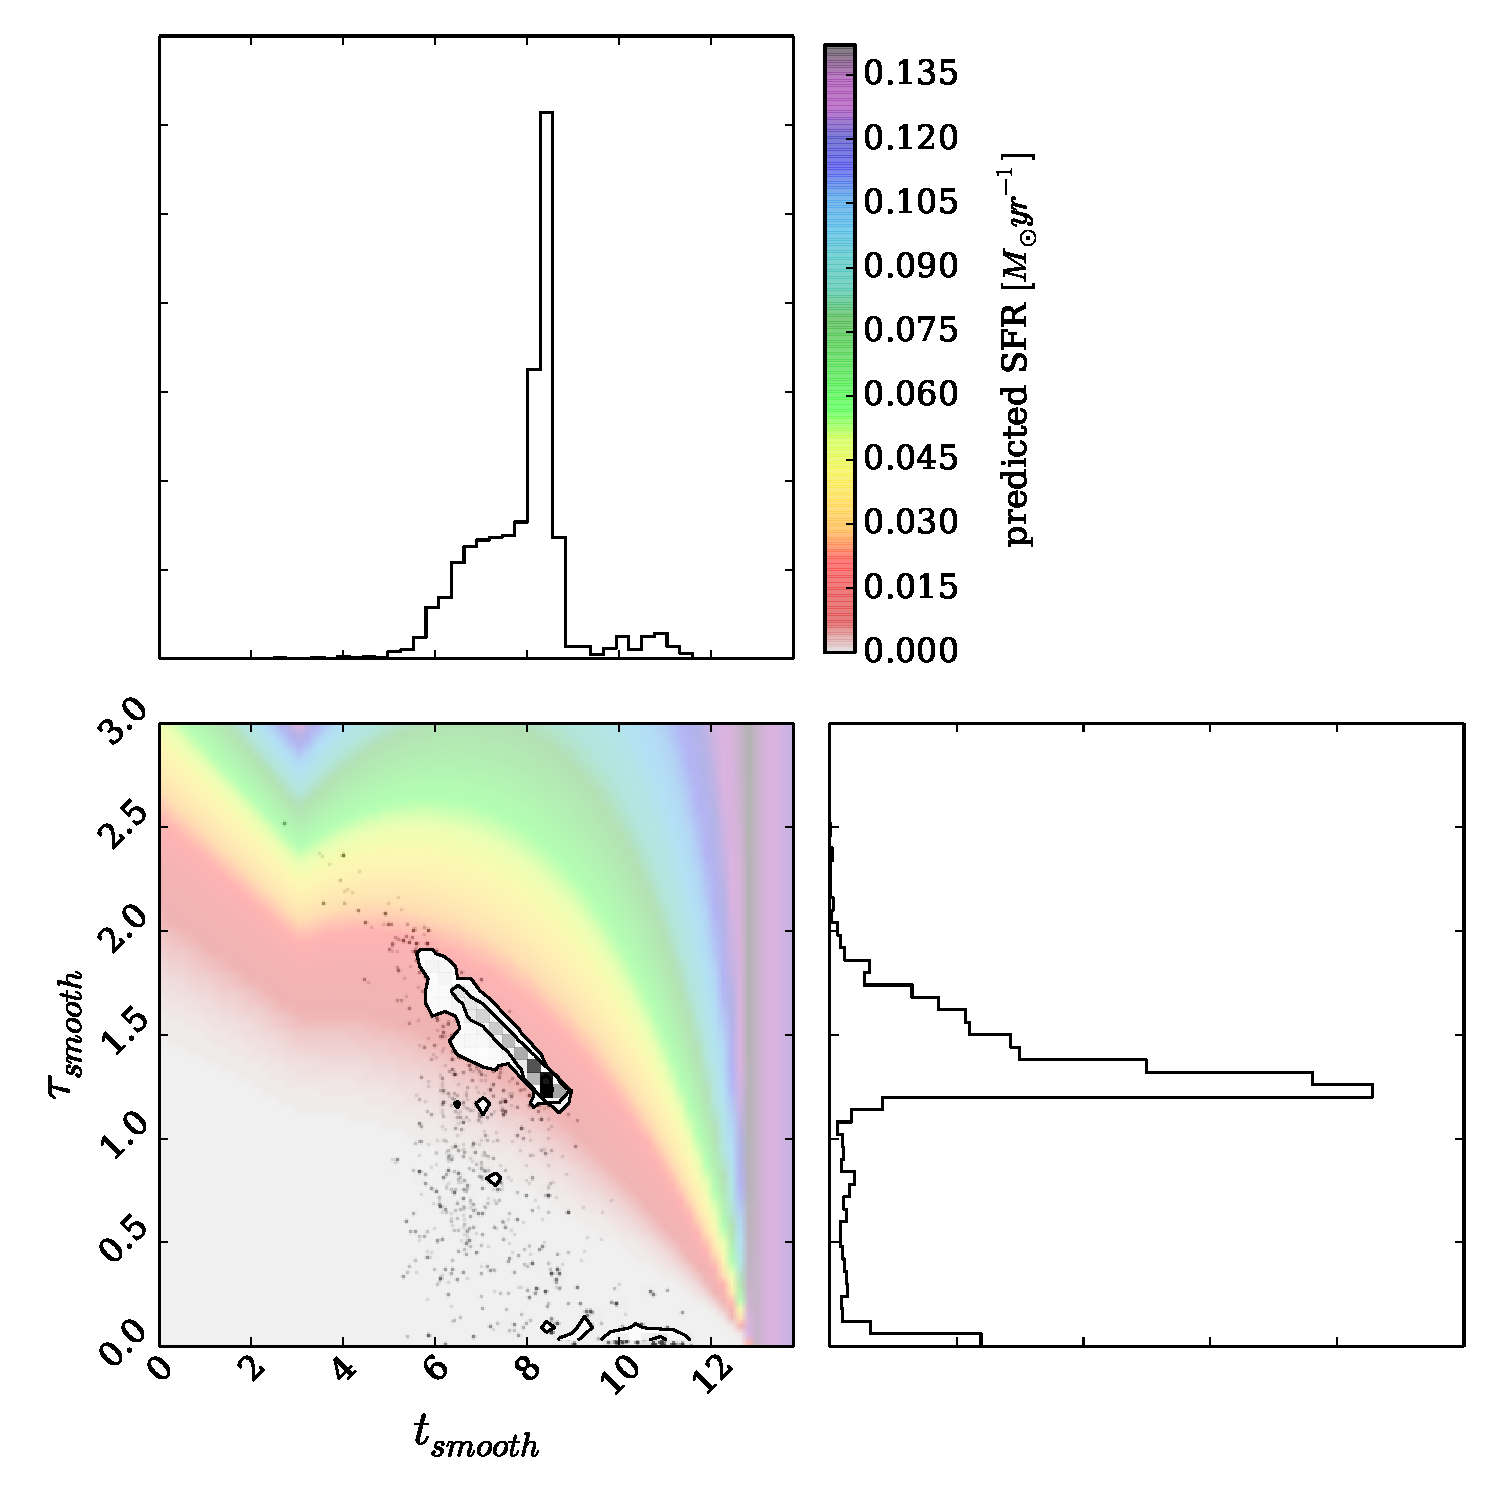
\includegraphics[width=0.4975\textwidth]{gv_smooth_clean.pdf}
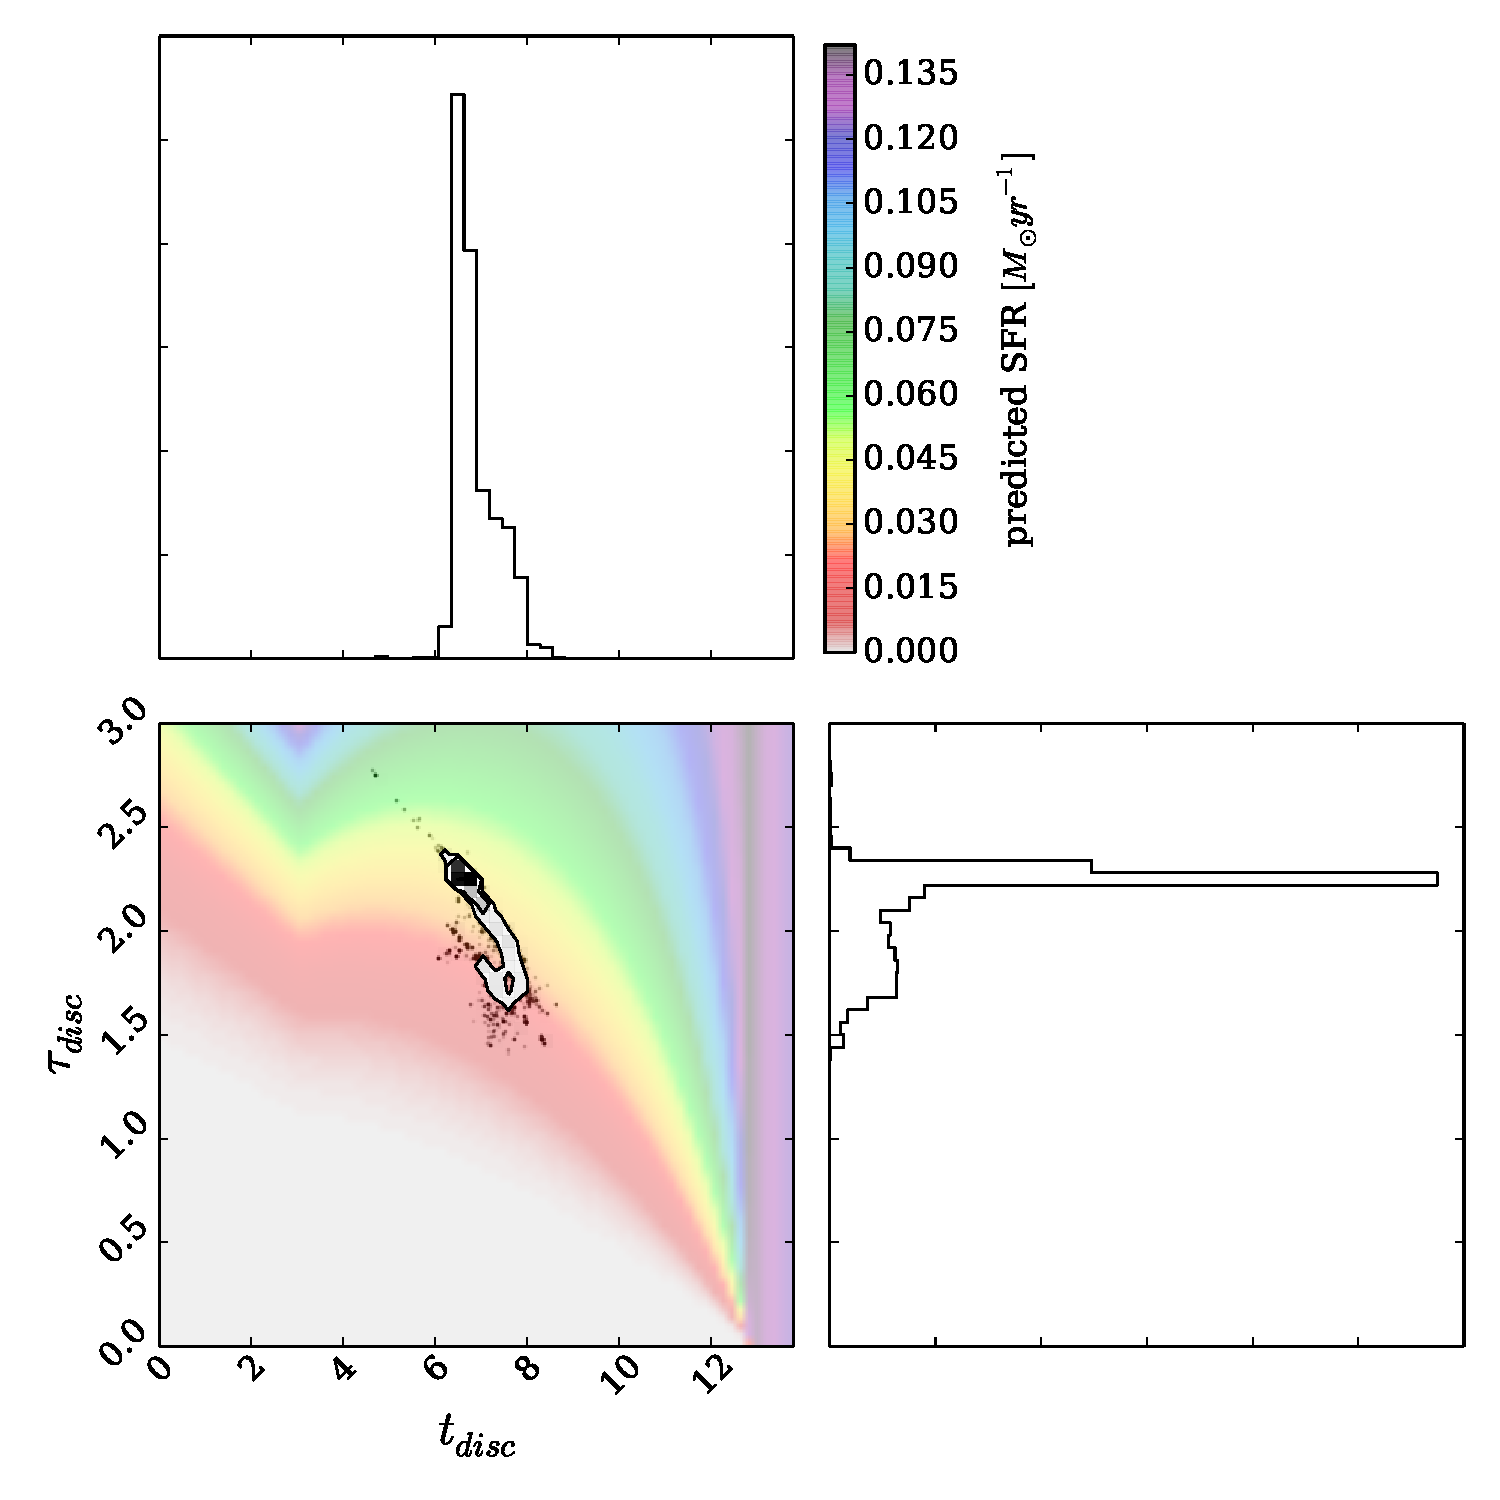
\includegraphics[width=0.4975\textwidth]{gv_disc_clean.pdf}
\caption{Same as for Figure \ref{all} but for galaxies from the clean sample and defined as optical Green Valley \cite{Baldry}.}
\label{gv_clean}
\end{figure*}


\begin{figure*}
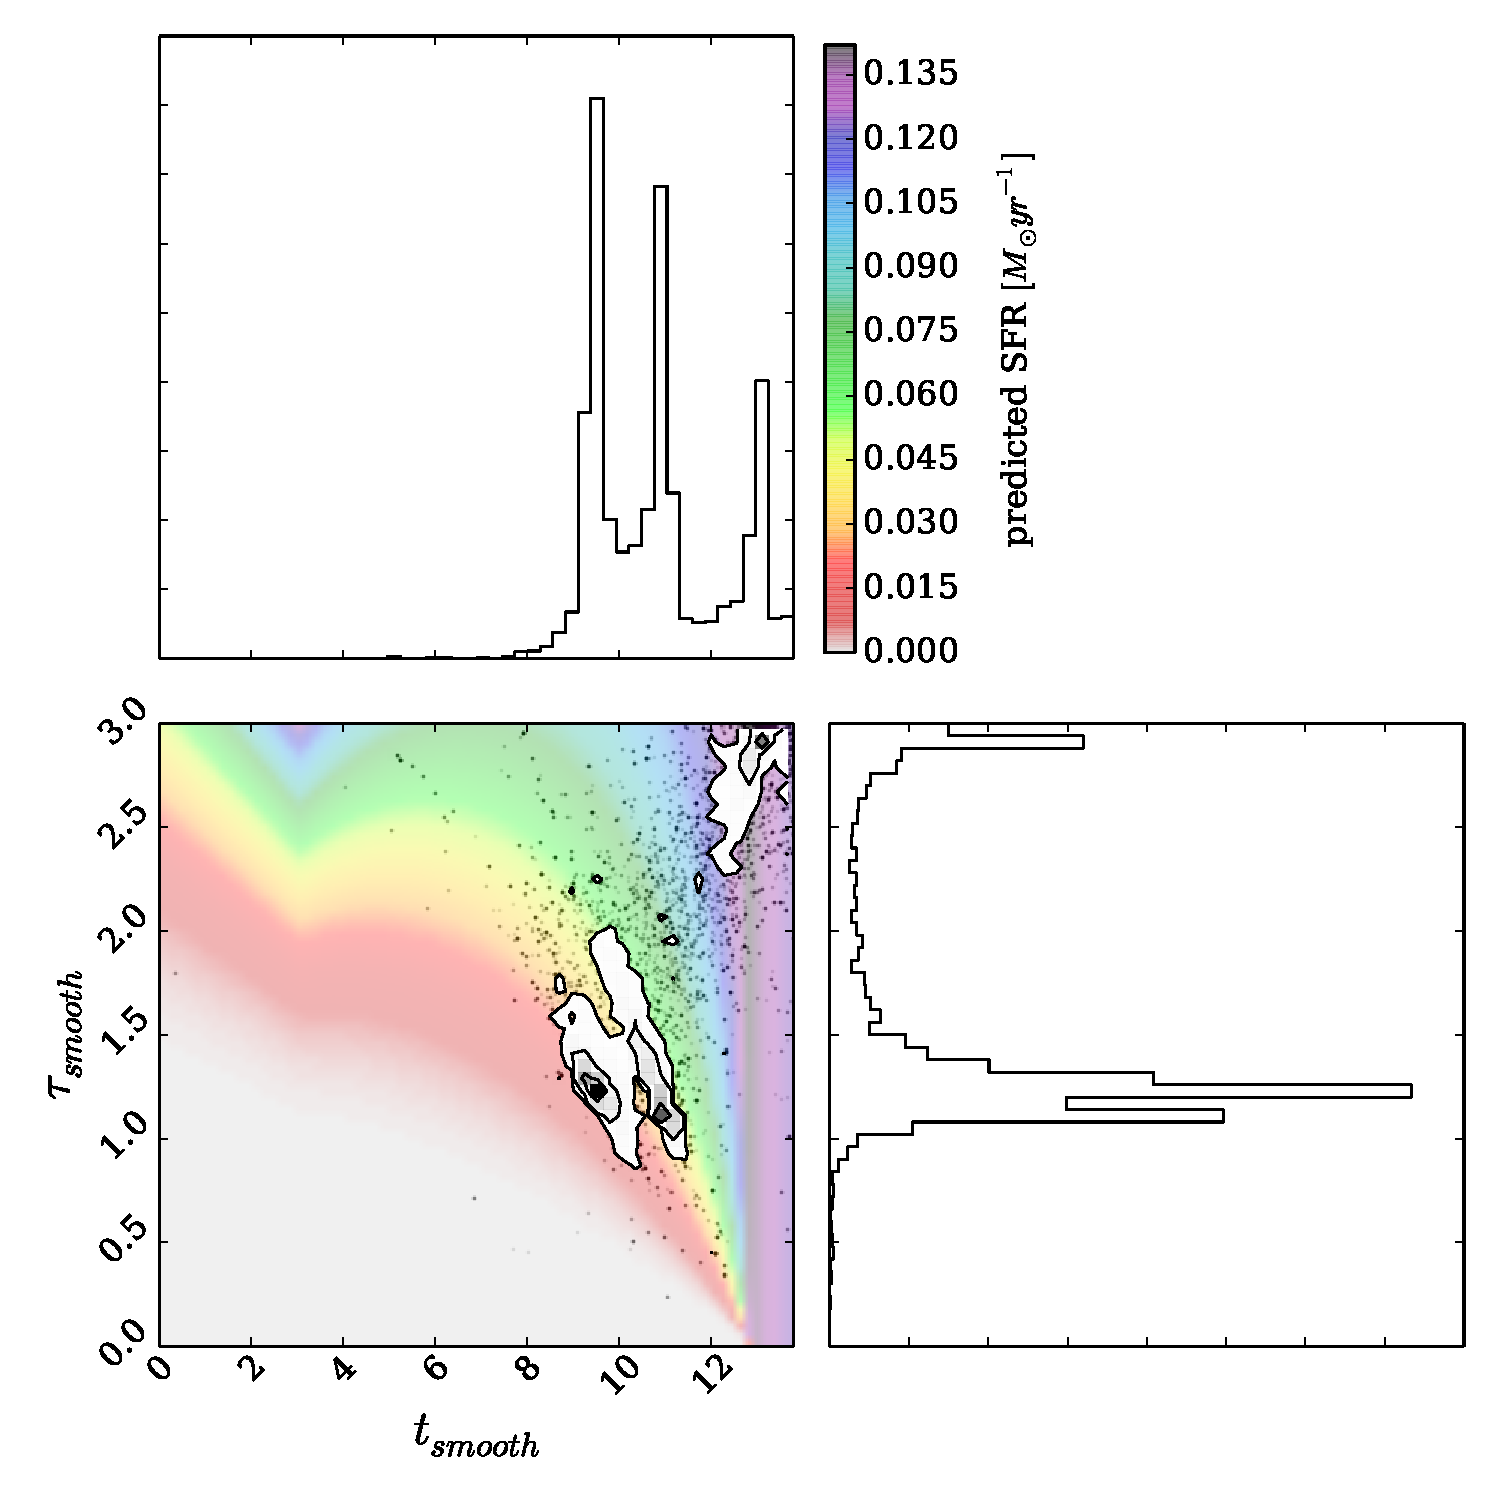
\includegraphics[width=0.4975\textwidth]{blue_c_smooth.pdf}
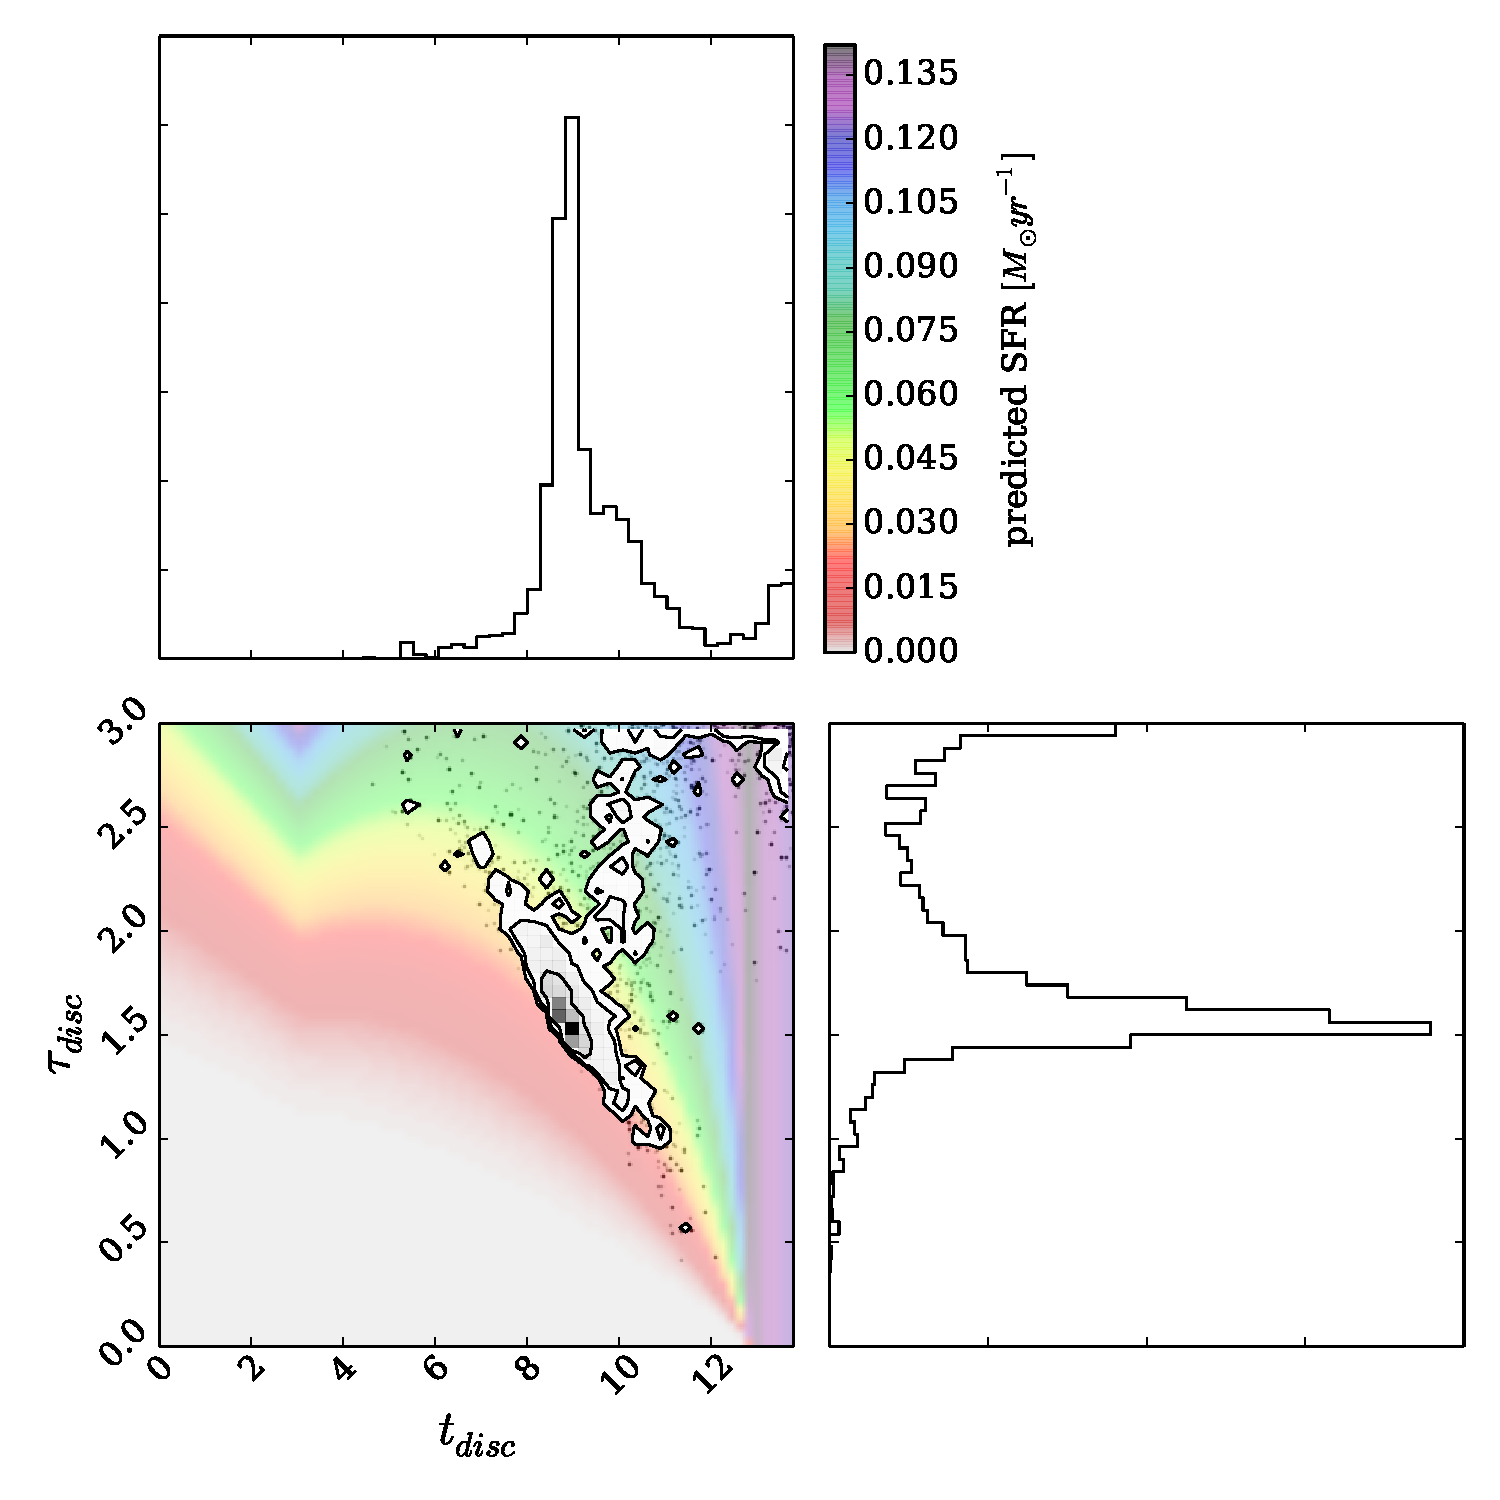
\includegraphics[width=0.4975\textwidth]{blue_c_disc.pdf}
\caption{Same as for Figure \ref{all} but for galaxies defined as optical Blue Cloud \cite{Baldry}.}
\label{blue_c}
\end{figure*}

\begin{figure*}
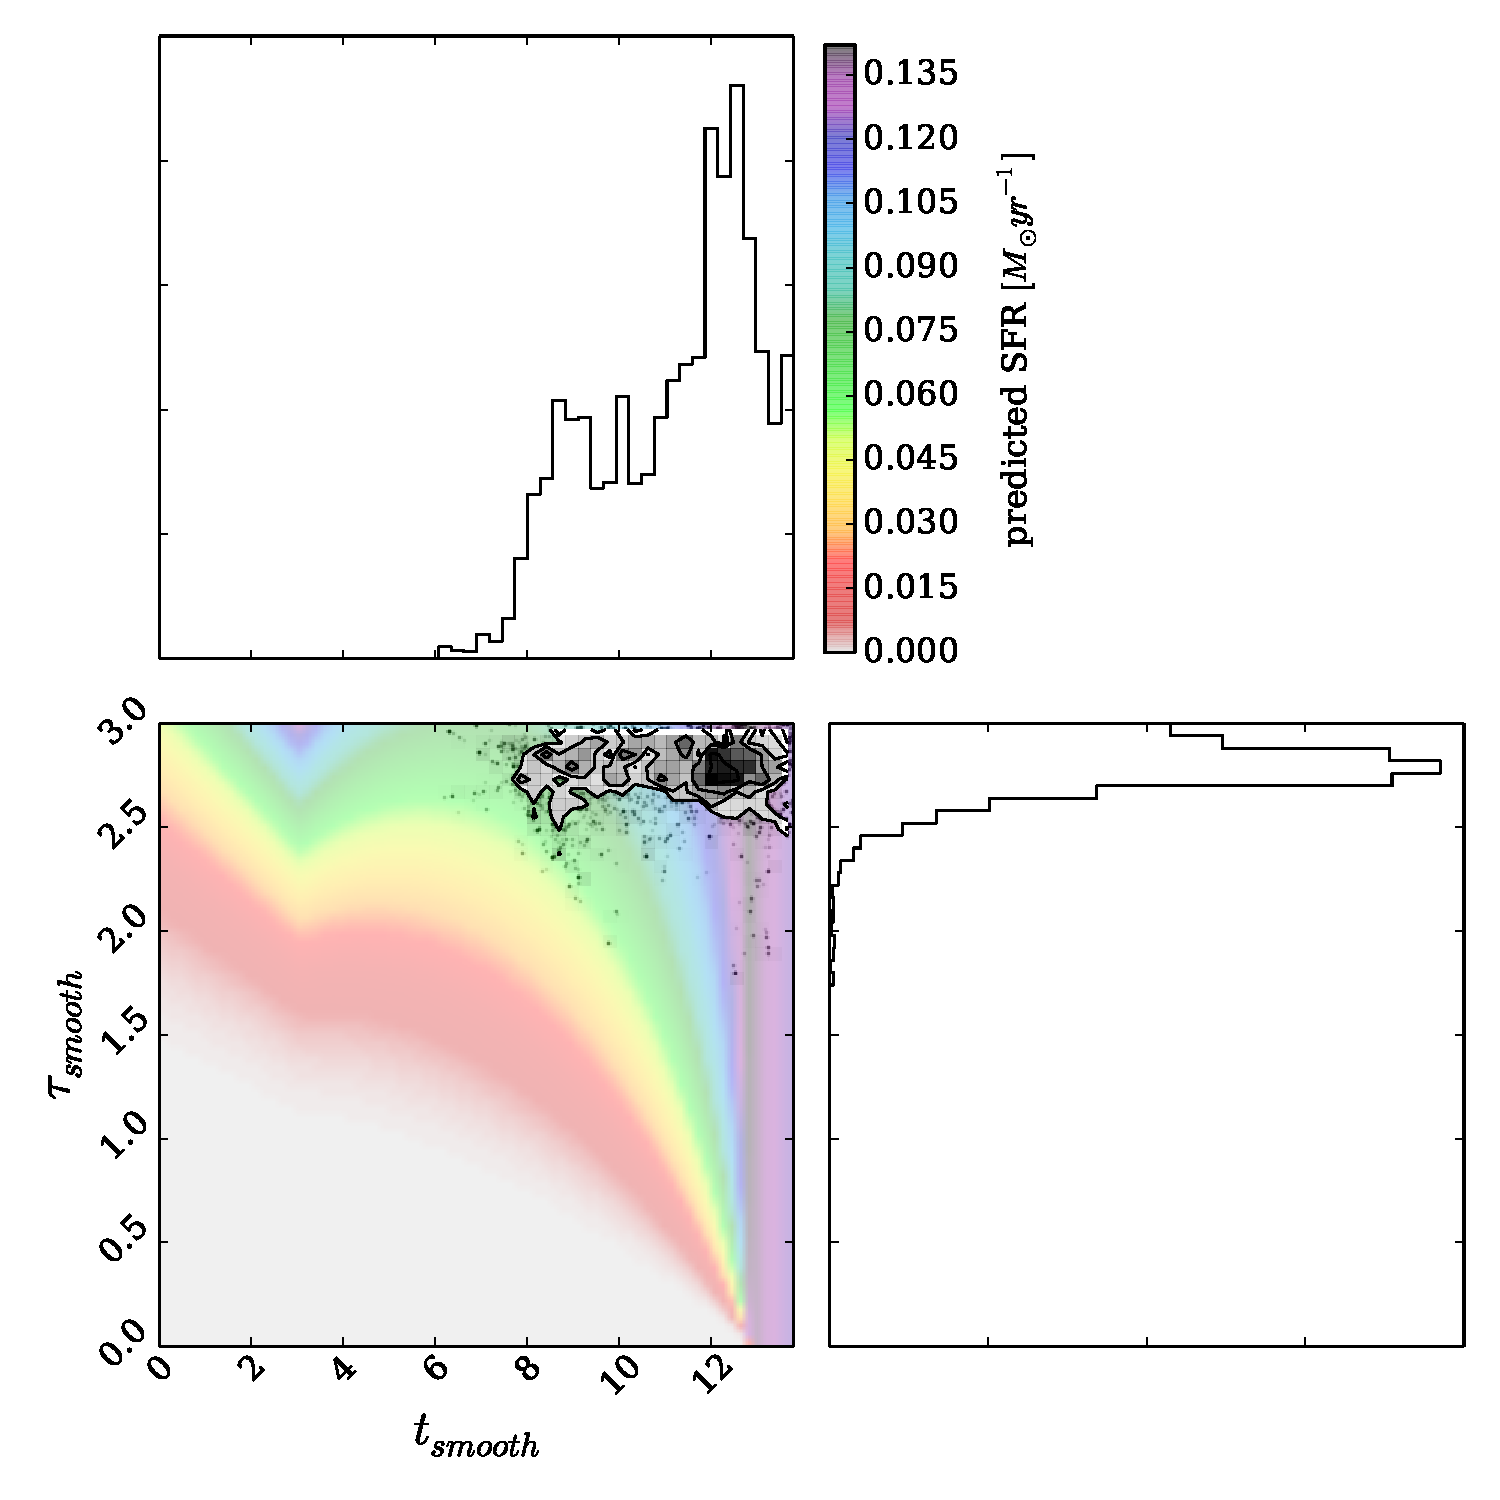
\includegraphics[width=0.4975\textwidth]{blue_c_smooth_clean.pdf}
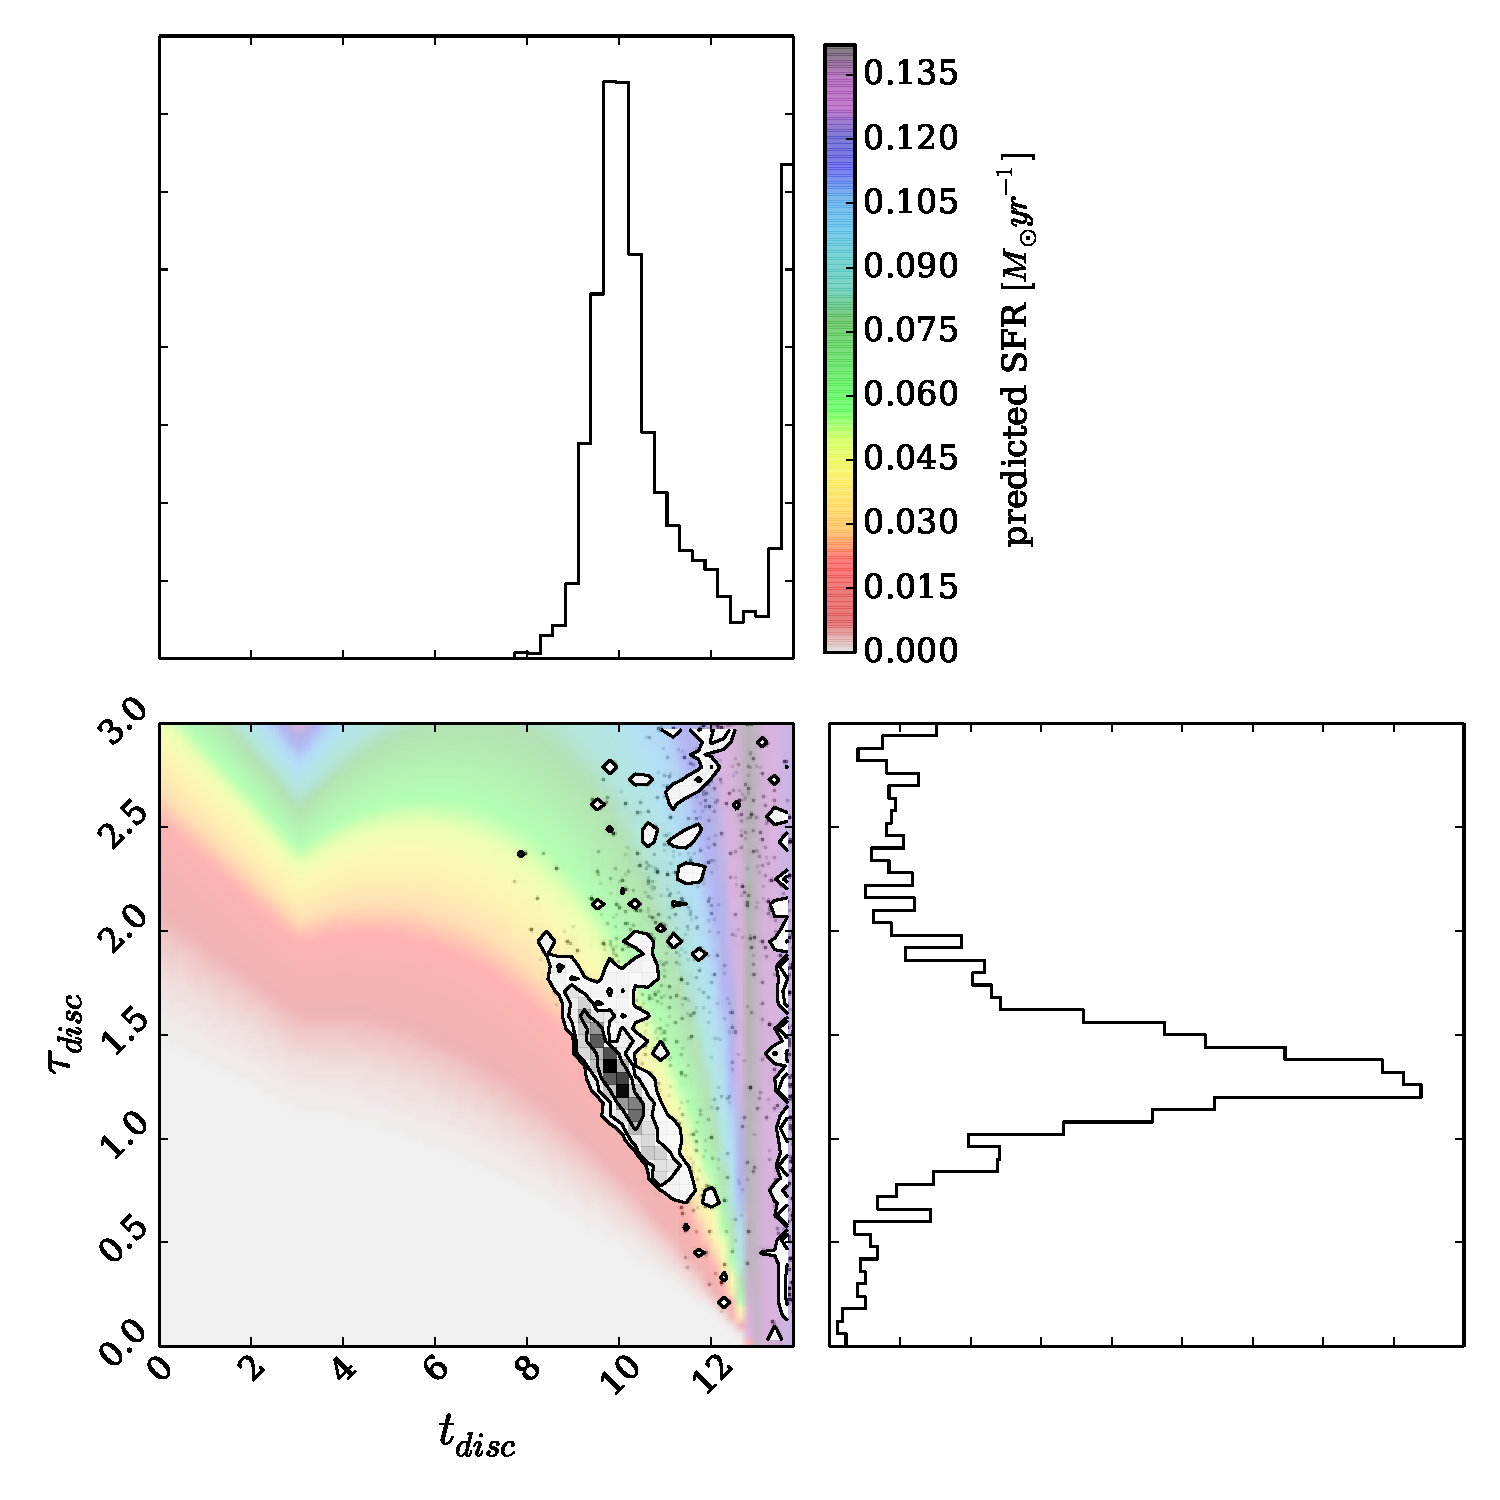
\includegraphics[width=0.4975\textwidth]{blue_c_disc_clean.pdf}
\caption{Same as for Figure \ref{all} but for galaxies from the clean sample and defined as optical Blue Cloud \cite{Baldry}.}
\label{blue_c_clean}
\end{figure*}

\begin{figure*}
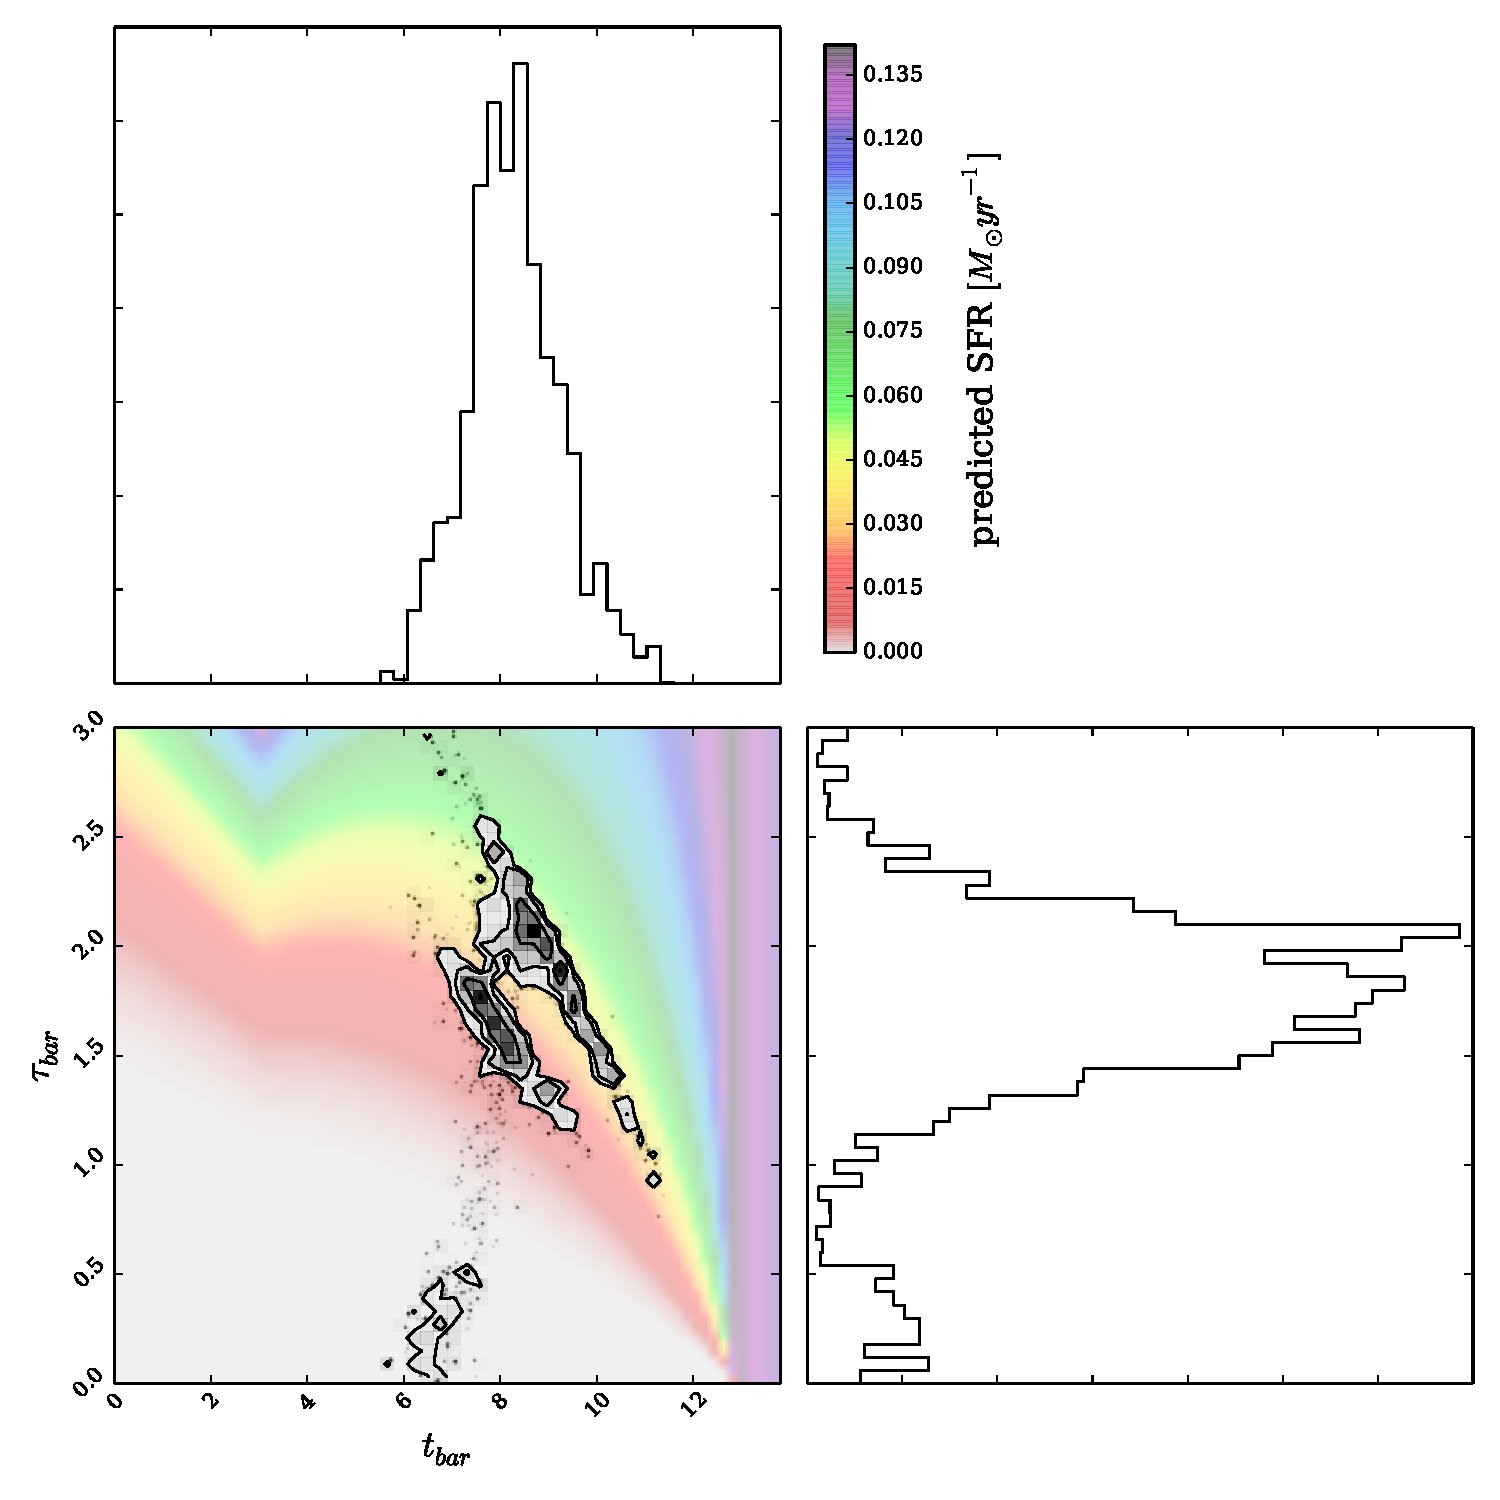
\includegraphics[width=0.4975\textwidth]{bars.pdf}
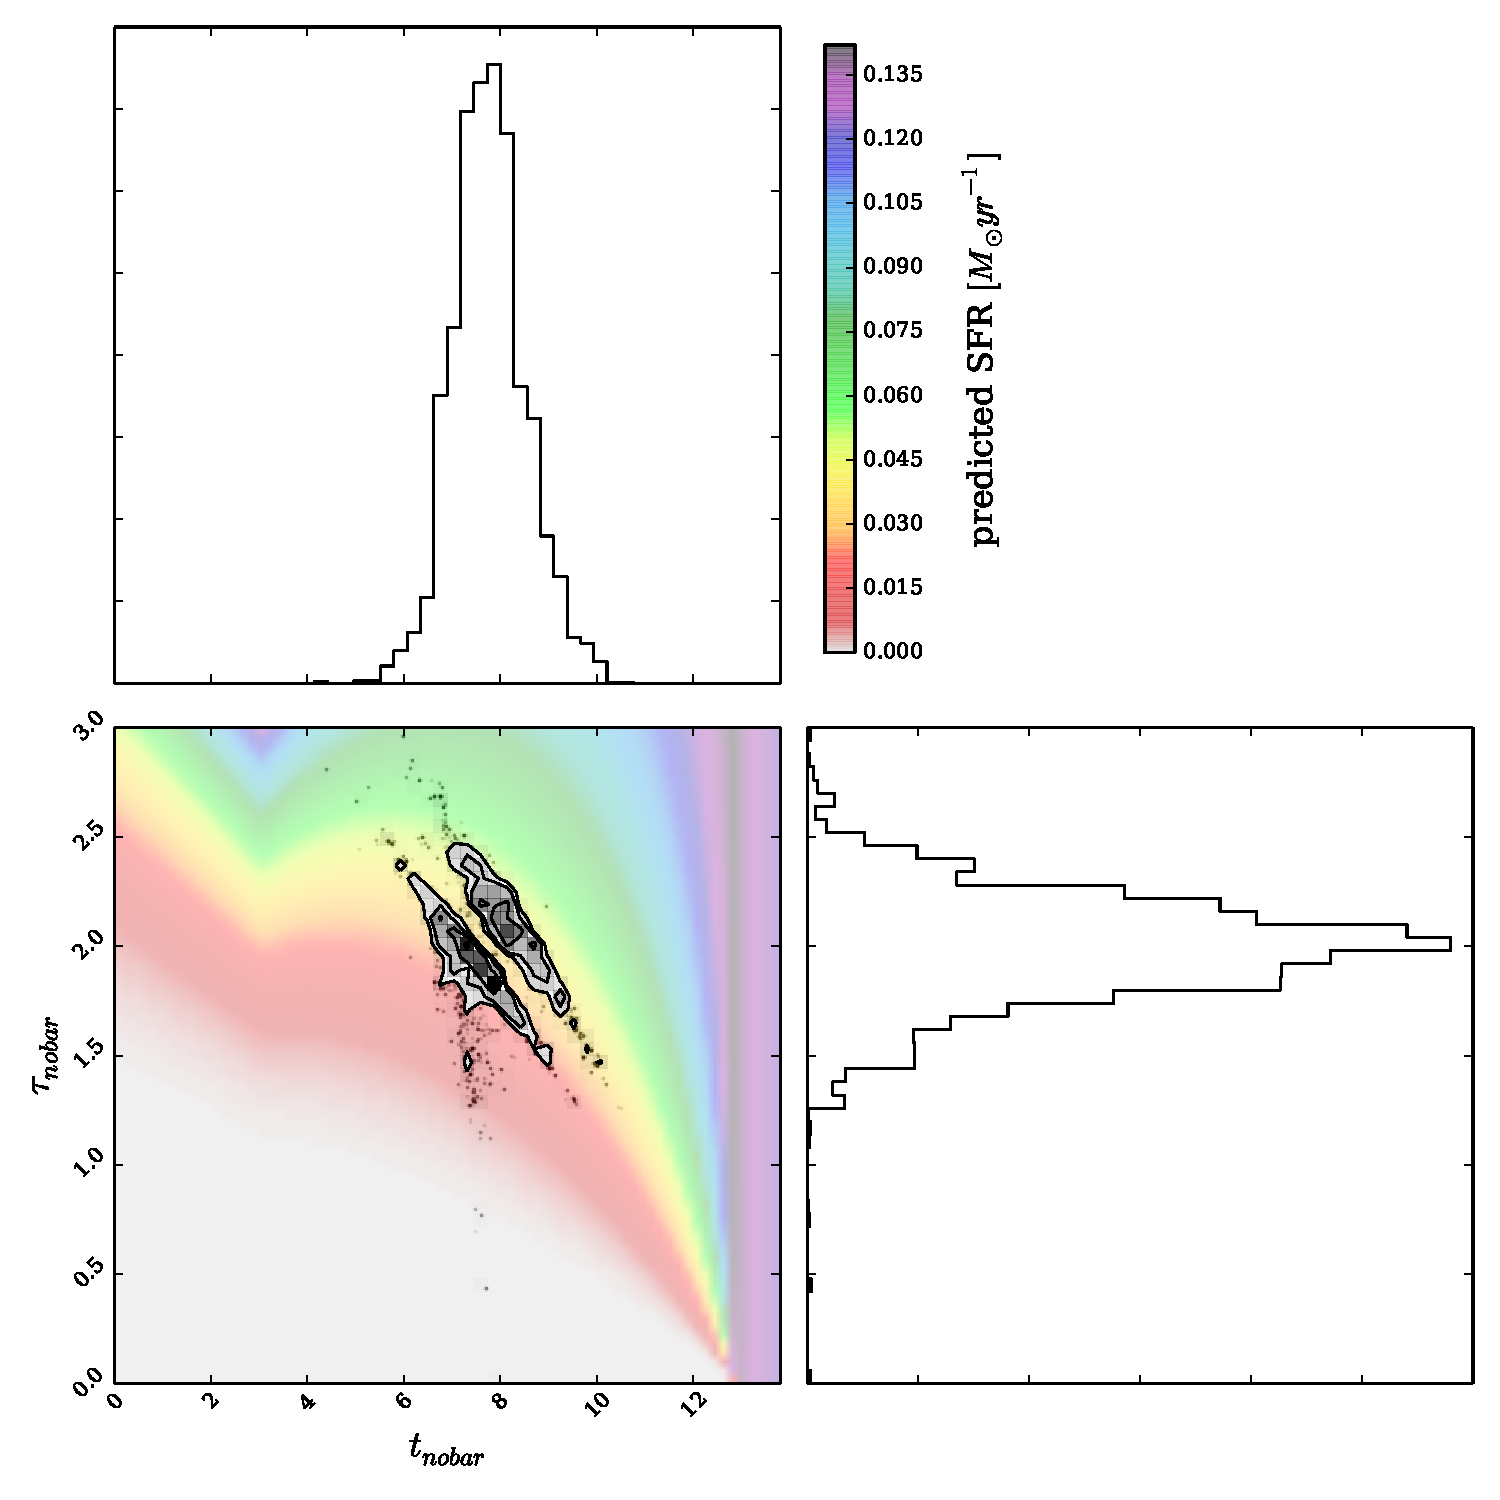
\includegraphics[width=0.4975\textwidth]{no_bars.pdf}
\caption{Same as for Figure \ref{all} but for barred and non barred galaxies.}
\label{bars}
\end{figure*}

\section{Discussion}
In figure \ref{all} we can immediately see that the two populations occupy very different locations in the $[t, \tau]$ parameter space supporting the conclusion in \citet{Sch2014} that early- and late- type galaxies have different quenching timescales. We can also see a significant \emph{correlation} between the two parameters $[t, \tau]$ (if quenching occurs earlier, then the quenching timescale increases) particularly for the disc-like galaxies. 

For the disc-like galaxies we have a bimodal likelihood in the SFH parameter space, whereas for the smooth-like galaxies we have a trimodal likelihood. For the disc galaxies we see no likelihood below $\tau \sim 1~Gyr$ (rapid quenching), whereas we do see an area of likelihood for the smooth galaxies - most likely caused by typical massive, red early type galaxies. The likelihood for $t_{quench}$ for the disc-like galaxies spans a much larger range than for the smooth-like galaxies and also has a correlation with $\tau$; when quenching occurs at an earlier time, the quenching timescale is much longer, whereas when quenching occurs at a later time, the quenching timescale is quicker. Perhaps this is due to a dependancy on the environment which galaxies occupied at earlier times compared to later times. 

In figure \ref{red_s} we can see. defined to be in the optical Red Sequence, a prevalence for fast quenching timescales for the smooth-like galaxies and slow quenching timescales for the disc-like galaxies ; again confirming the results found by \citet{Sch2014}. However there is also a significant likelihood for blue NUV colours in the smooth parameters (slow quenching at late timescales) and for red NUV colours in the disc parameters. Could this be due to:
\begin{enumerate}[i] 
\item a population of S0 galaxies (with GZ2 likelihoods $p_s \sim p_d \sim 0.5$) which contribute to both sets of parameters? 
\item bulge dominated disc galaxies impacting on the likely disc parameters?
\item NUV blue smooth galaxies impacting on the likely smooth parameters? 
\end{enumerate}
We can compare figure \ref{red_s} with figure \ref{red_s_clean} which shows the SFH parameters but only for those galaxies defined to be both in the optical Red Sequence and the GZ2 `clean' sample (i.e. $p_d \geq 0.8$ and $p_s \geq 0.8$). This enables us to disentangle which galaxies are contributing to which areas of high likelihood in figure \ref{red_s}. We can therefore see that the typical clean, smooth, red sequence galaxy has undergone a SFH with a relatively rapid quench at various times, resulting in a very low current SFR. These are therefore the typical \emph{`red and dead'} galaxies expected to be found in the red sequence. As for the clean disc  galaxies in the red sequence, presumably red spiral galaxies, there is no region of the parameter space which has a preferred likelihood, suggesting that although these disc galaxies are optically red, they have a wide range of NUV-u colours, giving rise to a wide range of timescales for the most recent episode star formation episode. This suggests that there is no `typical' red sequence disc galaxy and that there are many possible routes for a disc galaxy to the red sequence. 

In figures \ref{gv} and \ref{gv_clean} we can make similar comparisons as above but for the Green Valley galaxies. In figure \ref{gv} we still see the correlation between the two parameters as for all of the galaxies but the areas of high likelihood for the parameters has changed. We have a very clear bimodal likelihood in the parameter space for smooth galaxies; this is also slightly apparent in the likelihoods for the parameters for the disc-like green valley galaxies, but is not as pronounced. If we compare this to figure \ref{gv_clean} we can see that this bimodaility has disappeared for both smooth- an disc- like populations. This suggests that there are not just two routes for galaxies through the green valley but \emph{three}: with the smooth, intermediate (e.g. S0 galaxies) and disc galaxies each having different SFHs which cause them to traverse across the Green Valley.

We can also see that quenching for the Green Valley occurs on longer quenching timescales; there is little to no likelihood for $\tau$ below $\sim 1.0 ~Gyr$ for the disc galaxies, however a small likelihood for recent rapid quenching of the smooth galaxies. This may be counter intuitive at first, as one of the main arguments for the lack of galaxies in the green valley is due to the hypothesised rapid movement across it; however, if this is the case then the expected number of galaxies in this region with this type of SFH (rapid quenching) is very small. It is remarkable therefore that we have managed to find some likelihood for this type of SFH in the parameter space (as seen in the left hand panel of figure \ref{gv}), however only for the smooth-like galaxies, suggesting that it is only early-type galaxies which traverse the green valley in this manner. The disc galaxies come to reside in the green valley after a relatively slow quench causing a transition from the centre to the edge of the blue cloud and eventually into the green valley. 

In figure \ref{blue_c} there is a preference for slow quenching at late times for both smooth- and disc-like galaxies but in this case we see a bimodality (or trimodality) in both populations, this time more strongly in the disc galaxies, compared to figure \ref{all}. The disc-like galaxies show a much stronger preference for slow quenching at late times than the smooth-like parameters, typically galaxies in the blue cloud will generally be galaxies whose only SFH to date has been some varying rate of star formation since it's formation with no quenching to date. There is also high likelihood in both samples for middle rate quenching at relatively recent times which could account for those galaxies on the edge of the blue cloud which have begun to quench. The SFH parameter space for the smooth-like and disc-like galaxies are very similar, suggesting that galaxies in the blue cloud are all very similar, regardless of morphology. \emph{I'm still not sure how this compares to the clean sample of blue cloud galaxies in figure \ref{blue_c_clean}, leave it with me...}

In figure \ref{bars} we can compare the star formation history parameters for barred and unbarred galaxies, selected so that $N_{count, bar} > 10$ and $N_{count, no bar} > 10$. The analysis was then run with $p_{bar}$ and $p_{no bar}$ in place of $p_{smooth}$ and $p_{disc}$. We can see that two the populations occupy different areas in the SFH parameter space suggesting that bars have undergone a different formation history to non barred disc galaxies.  Barred galaxies simultaneously are more likely to have bluer and redder colours than non barred galaxies, as the bimodality seen in the SFH parameters of the non barred galaxies in the right hand panel of figure \ref{bars} has moved outwards. This suggests that the argument for whether bars promote or quench star formation rates in galaxies could have evidence for both possibilities. Perhaps the amount and distribution of gas present in a galaxy prior to the formation of the bar determines what effect the bar will have on the star formation rate. There is also a region of likelihood at very rapid quenching timescales for barred galaxies which is not present in the parameters for the non barred galaxies, supporting the hypothesis that bars turn galaxies red (\emph{cite Maraston papers here}). To explain what we see here we can say either that:
\begin{enumerate}[i]
\item As a bar forms it can cause a rapid quenching of star formation in it's host galaxy,
\item A rapid quenching of star formation in a galaxy can cause a bar to form.
\end{enumerate}
This analysis however, does not allow for this to be determined. 

\section{Conclusion}
The three most important points: 
\begin{enumerate}[i]
\item There is a clear correlation between $t_{quench}$ and $\tau$. At earlier times, the quenching timescale is longer, whereas at more recent times, the quenching timescale is shorter on average. Could this be an environmental dependance of quenching with cosmic time?
\item There are a wide range of possible routes to the red sequence for disc galaxies. Some have similar SFHs to the red sequence smooth galaxies, whereas some have similar SFHs to blue cloud disc galaxies. Morphology seems to be irrelevant to the SFH. 
\item There are three possible routes through the green valley dependant on morphology. 
\end{enumerate}

There is not one specific route to each part of the colour-colour or colour-magnitude diagram, due to the complex interplay between the SFH parameters, however the morphology of a galaxy can have varying impacts and constraints on what these parameters can be.

\begin{thebibliography}{}
\bibitem[\protect\citeauthoryear{Baldry et al. }{2004}]{Baldry} Baldry, I. K. et al., 2004, ApJ, 600, 681
\bibitem[\protect\citeauthoryear{Bruzual \& Charlot }{2003}]{BC03} Bruzual, G. \& Charlot, S., 2003, MNRAS, 344, 1000
\bibitem[\protect\citeauthoryear{Foreman-Mackey et al. }{2013}]{Dan} Foreman-Mackey, D., Hogg, D. W., Lang, D., Goodman, J., 2013, PASP, 125, 306
\bibitem[\protect\citeauthoryear{Peng et al. }{2010}]{Peng} Peng, Y. et al., 2010, ApJ, 721, 193
\bibitem[\protect\citeauthoryear{Schawinski et al. }{2014}]{Sch2014} Schawinski, K. et al., 2014 (arXiv: 1402.4814)
\bibitem[\protect\citeauthoryear{Willett et al. }{2013}]{GZ2} Willett, K. et al., 2014, MNRAS, 435, 2835
\end{thebibliography}
\end{document}
